%% 使用 njuthesis 文档类生成南京大学学位论文的示例文档
%%
%% 作者:胡海星,starfish (at) gmail (dot) com
%%
%%
\documentclass[master,winfonts]{njuthesis}
%% njuthesis 文档类的可选参数有:
%%   nobackinfo 取消封二页导师签名信息。注意,按照南大的规定,是需要签名页的。
%%   phd/master/bachelor 选择博士/硕士/学士论文

% 使用 blindtext 宏包自动生成章节文字
% 这仅仅是用于生成样例文档,正式论文中一般用不到该宏包
\usepackage[math]{blindtext}
%%\usepackage[caption=false]{subfig}
%\usepackage{subcaption}
\usepackage{subfig}
\usepackage{amsmath}
\usepackage{url}

% 论文的密级。需按照GB/T 7156-2003标准进行设置。预定义的值包括:
% - \openlevel,表示公开级:此级别的文献可在国内外发行和交换。
% - \controllevel,表示限制级:此级别的文献内容不涉及国家秘密,但在一定时间内
%   限制其交流和使用范围。
% - \confidentiallevel,表示秘密级:此级别的文献内容涉及一般国家秘密。
% - \clasifiedlevel,表示机密级:此级别的文献内容涉及重要的国家秘密 。
% - \mostconfidentiallevel,表示绝密级:此级别的文献内容涉及最重要的国家秘密。
% 此属性可选,默认为\openlevel,即公开级。
\securitylevel{\controllevel}
%%%%%%%%%%%%%%%%%%%%%%%%%%%%%%%%%%%%%%%%%%%%%%%%%%%%%%%%%%%%%%%%%%%%%%%%%%%%%%%
% 设置论文的中文封面

% 论文标题,不可换行
\title{基于计算机视觉的零件表面缺陷检测研究和应用}
% 如果论文标题过长,可以分两行,第一行用\titlea{}定义,第二行用\titleb{}定义,将上面的\title{}注释掉
\titlea{基于计算机视觉的零件表面}
\titleb{缺陷检测研究和应用}
% 论文作者姓名
\author{宋佳}
% 论文作者联系电话
\telphone{15251836269}
% 论文作者电子邮件地址
\email{sjbetter@163.com}
% 论文作者学生证号
\studentnum{MG1533047}
% 论文作者入学年份(年级)
\grade{2015}
% 导师姓名职称
\supervisor{郭延文~~教授}
% 导师的联系电话
\supervisortelphone{13913028596}
% 论文作者的学科与专业方向
\major{多媒体}
% 论文作者的研究方向
\researchfield{计算机视觉}
% 论文作者所在院系的中文名称
\department{计算机科学与技术系}
% 论文作者所在学校或机构的名称。此属性可选,默认值为``南京大学''。
\institute{南京大学}
% 论文的提交日期,需设置年、月、日。
\submitdate{2018年5月10日}
% 论文的答辩日期,需设置年、月、日。
\defenddate{2018年5月14日}
% 论文的定稿日期,需设置年、月、日。此属性可选,默认值为最后一次编译时的日期,精确到日。
%% \date{2013年5月1日}

%%%%%%%%%%%%%%%%%%%%%%%%%%%%%%%%%%%%%%%%%%%%%%%%%%%%%%%%%%%%%%%%%%%%%%%%%%%%%%%
% 设置论文的英文封面

% 论文的英文标题,不可换行
\englishtitle{A research of defect detection on the surface of parts based on computer vision and its application}
% 论文作者姓名的拼音
\englishauthor{Jia Song}
% 导师姓名职称的英文
\englishsupervisor{Professor Yanwen Guo}
% 论文作者学科与专业的英文名
\englishmajor{Multimedia}
% 论文作者所在院系的英文名称
\englishdepartment{Department of Computer Science and Technology}
% 论文作者所在学校或机构的英文名称。此属性可选,默认值为``Nanjing University''。
\englishinstitute{Nanjing University}
% 论文完成日期的英文形式,它将出现在英文封面下方。需设置年、月、日。日期格式使用美国的日期
% 格式,即``Month day, year'',其中``Month''为月份的英文名全称,首字母大写;``day''为
% 该月中日期的阿拉伯数字表示;``year''为年份的四位阿拉伯数字表示。此属性可选,默认值为最后
% 一次编译时的日期。
\englishdate{May 10, 2018}

%%%%%%%%%%%%%%%%%%%%%%%%%%%%%%%%%%%%%%%%%%%%%%%%%%%%%%%%%%%%%%%%%%%%%%%%%%%%%%%
% 设置论文的中文摘要

% 设置中文摘要页面的论文标题及副标题的第一行。
% 此属性可选,其默认值为使用|\title|命令所设置的论文标题
% \abstracttitlea{数据中心网络模型研究}
% 设置中文摘要页面的论文标题及副标题的第二行。
% 此属性可选,其默认值为空白
% \abstracttitleb{}

%%%%%%%%%%%%%%%%%%%%%%%%%%%%%%%%%%%%%%%%%%%%%%%%%%%%%%%%%%%%%%%%%%%%%%%%%%%%%%%
% 设置论文的英文摘要

% 设置英文摘要页面的论文标题及副标题的第一行。
% 此属性可选,其默认值为使用|\englishtitle|命令所设置的论文标题
\englishabstracttitlea{A research of defect detection on the surface of parts }
% 设置英文摘要页面的论文标题及副标题的第二行。
% 此属性可选,其默认值为空白
\englishabstracttitleb{based on computer vision and its application}

%%%%%%%%%%%%%%%%%%%%%%%%%%%%%%%%%%%%%%%%%%%%%%%%%%%%%%%%%%%%%%%%%%%%%%%%%%%%%%%
\begin{document}

%%%%%%%%%%%%%%%%%%%%%%%%%%%%%%%%%%%%%%%%%%%%%%%%%%%%%%%%%%%%%%%%%%%%%%%%%%%%%%%

% 制作国家图书馆封面(博士学位论文才需要)
%\makenlctitle
% 制作中文封面
\maketitle

% 制作英文封面
\makeenglishtitle


%%%%%%%%%%%%%%%%%%%%%%%%%%%%%%%%%%%%%%%%%%%%%%%%%%%%%%%%%%%%%%%%%%%%%%%%%%%%%%%
% 开始前言部分
%\frontmatter

%%%%%%%%%%%%%%%%%%%%%%%%%%%%%%%%%%%%%%%%%%%%%%%%%%%%%%%%%%%%%%%%%%%%%%%%%%%%%%%
% 论文的中文摘要
\begin{abstract}

近年来,计算机视觉和深度学习的不断进步取得了瞩目的成功,不仅在学术界中被广泛研究,在工业界中也被大量应用。
其中,目标检测是非常基础和经典的课题,
而缺陷检测则是目标检测极具工业价值的应用领域。
传统的缺陷检测算法通常首先提取图像中的特征,进而将特征作为分类器的输入对图像分类。
这类方法存在着特征选择要求严格,分类模型泛化能力较弱,
容易受成像效果、零件纹理、光照条件和噪声等因素影响的缺点。
此外,既有的基于深度学习的缺陷检测算法
一般也存在两个不可忽视的缺点,首先模型训练需要大量数据;
其次模型对小目标效果不理想,而在零件缺陷检测中,缺陷往往较小。
这些困难和挑战严重制约了缺陷检测在实际场景中的应用。

针对上述挑战和业界需求,
本文首先从硬件设计和算法设计两个角度出发,
提出基于光线反射原理计算零件表面法线的方法,
接着将其作为传统缺陷检测算法的输入,
取得了理想的效果。
我们还将法线图应用到深度学习算法中,对比和分析了二者的结果。
本文的主要工作和创新有:
\begin{enumerate}

\item 本文提出了一种零件表面法线提取算法,包括硬件设计与算法设计两部分内容。
算法使用不同方向光源下拍摄得到的零件照片作为输入,基于光线的反射原理计算零件表面法线。
首先,我们设计了一套硬件设备,该设备包括遮光模块、平台模块、灯光模块、拍照模块和控制模块五大模块,
这些模块将相机、步进电机、LED灯带、滑轨、偏光镜和滤光膜等不同硬件组合成一个整体,
可以捕获不同方向光源下的零件照片。
接着我们将设备得到的零件照片作为法线计算算法的输入,提取零件法线。
为了优化照片的质量,提高零件法线的精度,
在实施法线计算算法之前,
本文首先对相机进行校正,
并对方向光源产生的光线损失进行光线补偿。
校正算法包括白平衡校正、色彩校正、畸变校正。
补偿算法首先预存储一套补偿数据,接着利用它对新的照片进行补偿。
值得一提的是,我们的法线提取算法不仅可以用来获取零件表面法线,还可以用来获取其他材质的表面法线。

\item 本文将法线图作为缺陷检测算法的输入,
研究了该背景下的最优特征组合及基于Adaboost方法的强分类器组合,
对传统的缺陷检测算法进行了改进,
并在进行了充分的实验验证。
本文首先使用传统检测算法进行检测,算法包括数据预处理、特征提取、设计和训练分类器以及用分类器进行检测等步骤。
在数据预处理阶段,
我们首先使用零件主表面提取算法滤除照片中的无关背景,
接着使用数据增强的方法扩大数据规模。
在特征提取阶段,我们分别提取了Haar-like特征、图像梯度特征、LBP特征、GLCM特征、HOG特征等不同的图像特征,并分析了不同特征的分类效果,根据分类效果对特征进行组合,从而得到一组最优特征组合。
在分类器分类阶段,
由于缺陷零件较少,
导致样本分布不平衡,
我们使用随机抽样的方法将数据集划分为不同的子数据集,
使每个子数据集拥有平衡的样本分布。
在训练阶段,我们使用支持向量机作为基分类器,对于每个子数据集,我们训练多个不同的基分类器,并利用Adaboost的方法将其组合成一个强分类器,
最终每个子数据集得到一个强分类器。
在检测阶段,
我们将这些强分类器组合成级联检测器,进行缺陷检测。

\item 本文将法线图作为深度学习模型的输入,
实验了基于深度学习的缺陷检测算法。
本文首先使用滑动窗口的方式将法线图分割成不同的窗口,
接着使用分类模型对这些窗口做分类。
在准备数据阶段,我们使用与传统算法中相似的预处理方法对数据进行处理。
在模型设计阶段,我们针对零件缺陷检测问题调整和优化了模型。
在模型训练和检测阶段,我们同样将数据集划分为不同的子数据集,
每个子数据集训练一个模型,
并利用级联的方式将它们组成一个级联检测器。
最后本文还将深度学习模型的检测结果与传统检测方法的结果进行了对比,分析了二者各自的优缺点及原因。

\end{enumerate}
% 中文关键词。关键词之间用中文全角分号隔开,末尾无标点符号。
\keywords{法线图,缺陷检测,支持向量机,深度学习}
\end{abstract}

%%%%%%%%%%%%%%%%%%%%%%%%%%%%%%%%%%%%%%%%%%%%%%%%%%%%%%%%%%%%%%%%%%%%%%%%%%%%%%%

% 论文的英文摘要
\begin{englishabstract}

With the continuous development of computer vision and machine learning,
something has been changed.
In the fields of computer vision and machine learning, object detection is a very classical and basic subject, while defect detection plays an important role in related applications. 
The traditional object detection algorithm mainly involves two steps.
The first is to extract the artificial features designed in the image and the second is to classify the images with the features as input by a classifier.
There are two main disadvantages in this method, 
one is the difficulty of feature engineering, 
the other is that the performance of the classification model is susceptible to lighting, noise, texture of the part and other conditions.
With the vigorous development of deep learning, more and more different detection models is developed to detect objects, which have achieved ideal results in many fields, especially in competitions. 
However, those models always demand a mountain of samples and
are not good at detecting little objects while most of defections are very small.

To solve this problem, this paper takes the normal map as the input of defect detection for the first time. We do the defect detection with a traditional method combined SVM, Adaboost and Cascade and a state-of-the-art performance is acheived. We also take the normal map as input as convolutional neural network, and compare the results with traditional method's.
The main work and innovation of this article could be found as follows:

\begin{enumerate}
\item We propose a method to acquire the normal map of parts' surface and  design an equipment to acquire the method's inputs. 
This equipment includes a camera, LED light bars, a stepper motor and so many other components. 
All components are constituted into five models so that we could get required information,
and we put forward a method to compute the normal maps with the inputs collected by our equipment mentioned above.
To make up the imperfection of the capture equipment,
we add some corrections and enhancements before the normal map's computation.
Those are
color correction,
white balance correction,
distortion correction 
and light compensation.
\item 
We also do some experiments on traditional object detection methods with the normal maps extracted by us.
We extract many diffierent features form the normal maps such as Haar-like, LBP, GLCM, Gradient, HOG and others,
and the model's results and performances with those features as input are evaluated separately.
Then we combine those features according to the model's results and performances. 
Furthermore, a variety of ways are tried to get more data such as rotation and mirroring because of the rareness of defections on the parts.
And considering the imbalance of data between the parts with defections and those without defection, 
we divide the datasets into several subdatasets.
For each subdatasets,
we use the the method of Adaboost to train a more powerful classifier with the base learner trained by SVM, then we use Cascade to combine those classifier to detect defections.
\item At last, we make some experiments with deep learning models. 
First, we use the sliding windows to divide the original normal map into some smaller windows,
and do some data augmentation on those windows as before. 
We also divide the datasets into some subdatasets and train a model for each subdataset.
We combine those moodels with Cascade to detect defections.
We also analyse the results and performances of this model comparing to traditional methods'.
\end{enumerate}






% 英文关键词。关键词之间用英文半角逗号隔开,末尾无符号。
\englishkeywords{Normal map, Defect detection, SVM,Deep learning}
\end{englishabstract}


%%%%%%%%%%%%%%%%%%%%%%%%%%%%%%%%%%%%%%%%%%%%%%%%%%%%%%%%%%%%%%%%%%%%%%%%%%%%%%%
% 论文的前言,应放在目录之前,中英文摘要之后
%基本本我删掉了
%\begin{preface}
%\vspace{1cm}
%\begin{flushright}
%韦小宝\\
%2013年夏于南京大学
%\end{flushright}
%
%\end{preface}
%%%%%%%%%%%%%%%%%%%%%%%%%%%%%%%%%%%%%%%%%%%%%%%%%%%%%%%%%%%%%%%%%%%%%%%%%%%%%%%
% 生成论文目次
\tableofcontents

%%%%%%%%%%%%%%%%%%%%%%%%%%%%%%%%%%%%%%%%%%%%%%%%%%%%%%%%%%%%%%%%%%%%%%%%%%%%%%%
% 生成插图清单。如无需插图清单则可注释掉下述语句。
%\listoffigures

%%%%%%%%%%%%%%%%%%%%%%%%%%%%%%%%%%%%%%%%%%%%%%%%%%%%%%%%%%%%%%%%%%%%%%%%%%%%%%%
% 生成附表清单。如无需附表清单则可注释掉下述语句。
%\listoftables

%%%%%%%%%%%%%%%%%%%%%%%%%%%%%%%%%%%%%%%%%%%%%%%%%%%%%%%%%%%%%%%%%%%%%%%%%%%%%%%
% 开始正文部分
\mainmatter

%%%%%%%%%%%%%%%%%%%%%%%%%%%%%%%%%%%%%%%%%%%%%%%%%%%%%%%%%%%%%%%%%%%%%%%%%%%%%%%
% 绪论
\chapter{绪论}\label{chapter_introduction}

本章首先介绍本文的研究背景,引出课题的动机、目的以及研究意义,
接着介绍现有解决方案概况,
最后介绍本文的主要工作以及后续章节的内容安排。

\section{研究背景}

随着工业的发展,各种零件的需求量大幅度增长,但是在零件的自动化生产中,由于加工设备或环境等因素,不可避免的导致零件缺陷的出现。常见的零件缺陷有裂纹、起皮、拉线、划痕、凹坑、凸起、斑点、腐蚀等,严重的甚至会出现偏芯、气孔。这些缺陷零件一旦流出,不仅可能在高级的设备组装时被发现、召回和索赔,更有可能在设备实际使用中造成故障,甚至引发事故。因此,传统零件加工中通常雇佣大量工人使用肉眼检测缺陷,这种方法往往浪费大量人力、财力,仍然难以取得较好效果。如图
\ref{fig:changguilingjian}中列举了几种常见的金属零件,金属零件大部分呈环状,而缺陷往往就出现在这些环形区域的表面。
\begin{figure}[htbp]
\centering
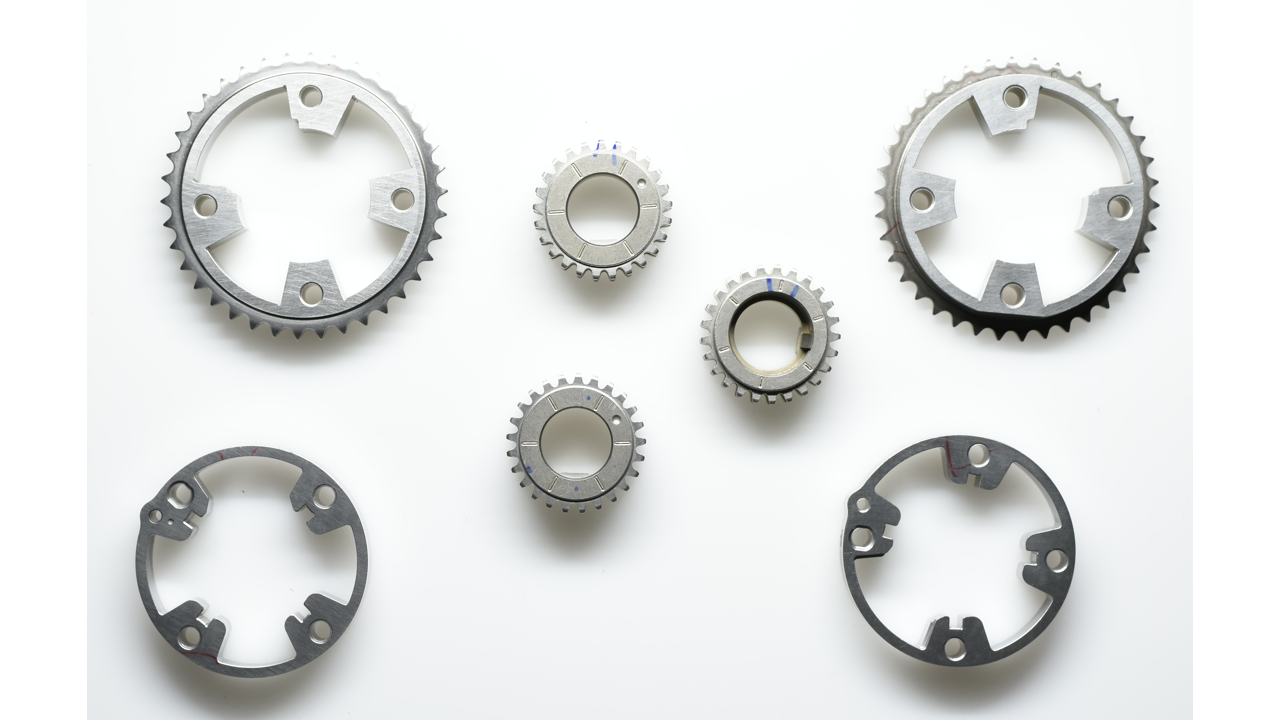
\includegraphics[width=0.8\textwidth]{figures/changguilingjian.png}\\
\caption{常规金属零件图}\label{fig:changguilingjian}
\end{figure}

在计算机视觉领域,缺陷检测是目标检测的一个重要应用。目标检测是通过计算机算法模拟人眼获取图片中感兴趣目标的过程,这一过程对于人类来说是一种本能,如同呼吸喝水一样简单,
但是对于计算机来说,
图片数据仅仅是$[0-255]$范围内的数字,
它很难理解这些信息所代表的含义,更分不清楚其中有什么物体以及这些物体所在的位置。
因此,对于计算机来讲,目标检测无疑是一项非常艰巨的任务。

传统的目标检测一般由获取原始图像、数据预处理、特征提取、训练分类器、使用分类器得到检测结果这几个步骤构成。其中特征提取是提取人工设计的特征,如梯度直方图\cite{dalal2005histograms}(Histogram of Oriented Gradients,简称 HOG)特征、
局部二值化\cite{ojala2000gray}(Local Binary Patterns,简称 LBP)特征
、
灰度共生矩阵\cite{haralick1973textural}(Gray-level Co-occurrence Matrix,简称GLCM)特征、
Oriented FAST and Rotated BRIEF\cite{rublee2011orb}(简称 ORB)特征等等。
传统分类模型主要包括决策树、支持向量机、逻辑斯特回归等。
这些分类器在某些问题上卓有成效,但是由于数据质量、特征设计、模型描述能力等因素限制,泛化能力有限,难以达到实际应用需要。
随着深度学习的发展,这类方法在分类和目标检测领域取得了非常好的效果,然而,这类模型要想取得较好结果,往往要求用海量数据对模型训练,并且动辄拥有上百层的网络结构,这种复杂的结构使得模型提取出的分类特征过于抽象,往往对于小目标难以取得较好效果,而在零件缺陷检测问题中,许多零件本身就不大,零件的缺陷则更小,深度学习往往难以奏效。

针对传统算法和深度学习算法的各自缺点,本文首先设计了提取零件法线图的方法,接着将法线图作为传统缺陷检测算法和深度学习缺陷检测算法的输入,进行缺陷检测,取得了理想的效果。

\section{现有工作概述}

在法线获取领域中,市面上最早出现的系统是
2013年Vizoo公司推出的Vizoo3D xTex,这是一款以相机为核心的表面信息提取系统,它通过相机对物体进行拍摄,然后使用一系列算法计算出材质的法线、
漫反射、高光以及透明度信息,是目前比较成熟的扫描系统,
但是该系统计算得到的法线并不精确。
目前国内也有
类似的系统,如厦门启尚科技研发的FSM 3D高清面料扫描仪,这款扫描仪小巧快
速,但是能够扫描的物体有限,并不能获取零件表面法线。

在目标检测领域,
传统的目标检测一般由获取原始图像、数据预处理、特征提取、训练分类器、使用分类器得到检测结果这几个步骤构成,如图\ref{chuantongjiancebuzhou}所示。
\begin{figure}[htbp]
\centering
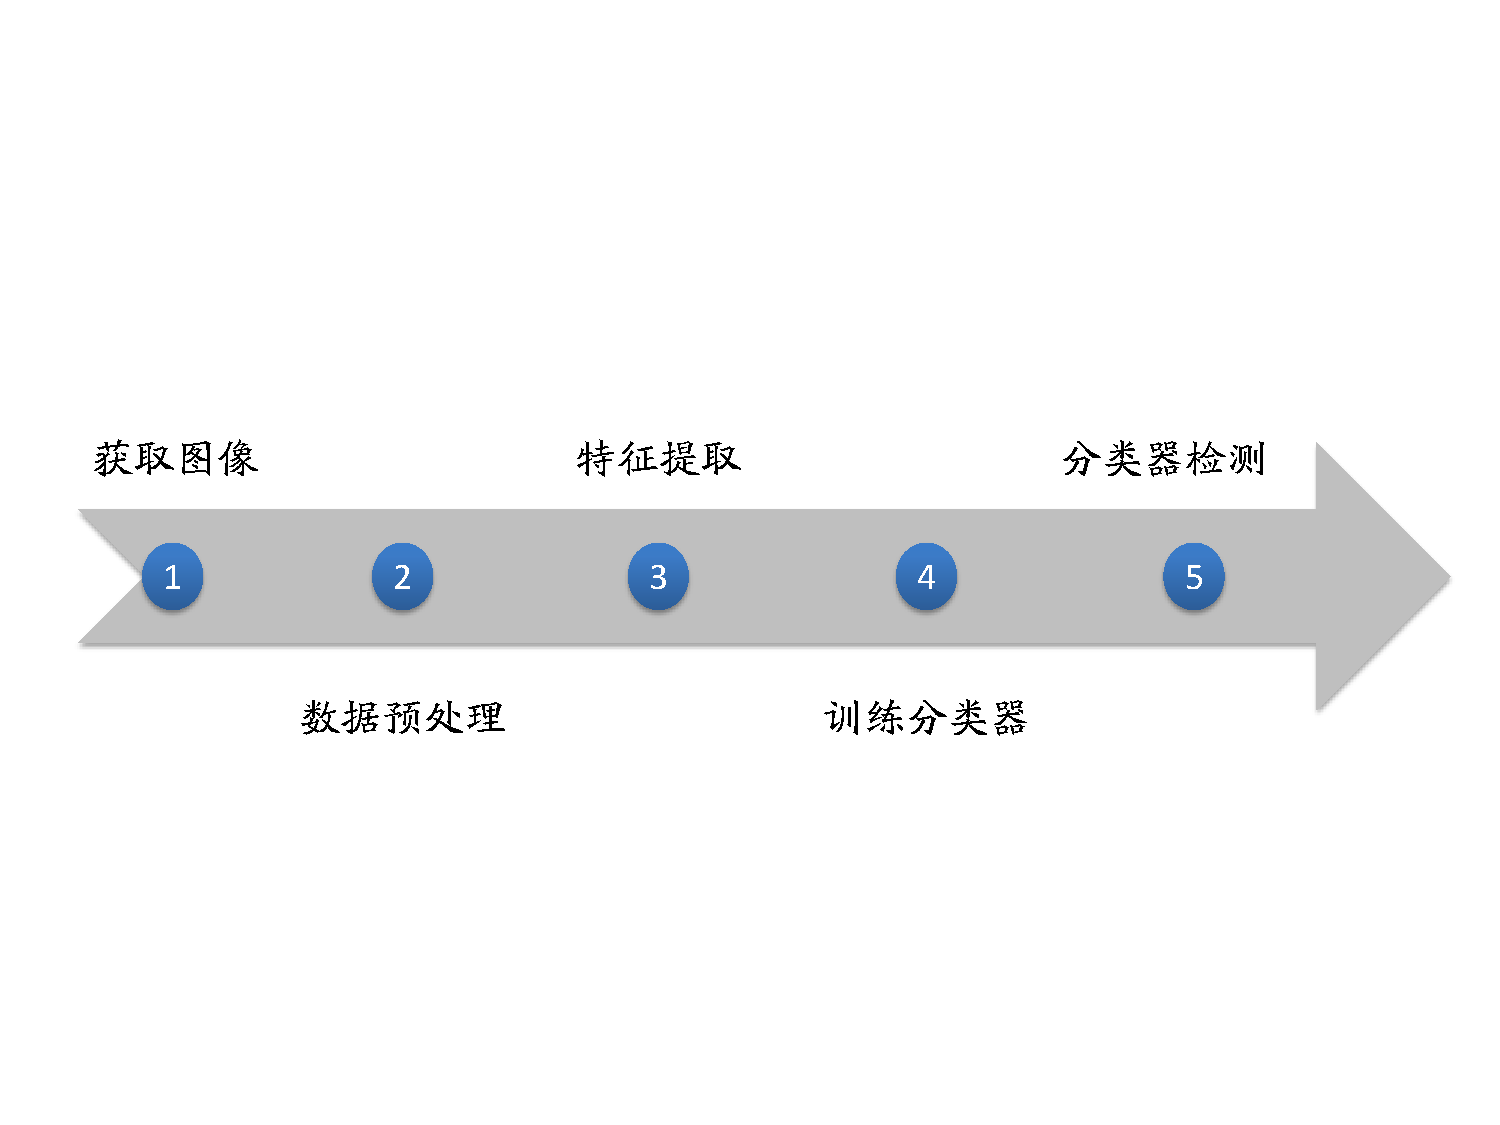
\includegraphics[width=1.0\linewidth]{figures/chuantongjiance.pdf}\\
\caption{传统方法缺陷检测步骤}\label{chuantongjiancebuzhou}
\end{figure}
在特征提取阶段,常用的特征有LBP特征、HOG特征、CLCM特征、哈尔\cite{viola2001rapid}(Haar-like)特征等等。
在分类器训练和检测阶段,一般采用不同尺寸的滑动窗口选择候选窗口用于训练和分类。
在分类器的选择中,
大多使用支持向量机\cite{hearst1998support}(Support Vector Machine,简称SVM)等传统的分类器模型。
其中,多尺度形变部件模型\cite{felzenszwalb2010object}(Deformable Part Mode,简称DPM)曾连续获得VOC(Visual Object Class)2007到2009的检测冠军,效果较好。
该算法将物体看成多个部件构成的整体,用部件之间的关系来描述物体,它继承了HOG和SVM各自的优点,但是模型的复杂度过高,检测速度不理想。

总的来说,传统的目标检测算法主要存在三个问题:
一是基于滑动窗口的窗口选择策略没有针对性,导致窗口冗余,时间复杂度过高;二是手工设计的特征往往对图片多样性的变化缺乏鲁棒性,并且在特征设计和选择阶段异常的复杂繁琐;三是分类模型往往泛化能力较弱。

自卷积神经网络\cite{lecun1998gradient}(Convolutional Neural Network, 简称 CNN)出现以来,产生了许多成熟的分类框架,其中最具代表性的有LeNet\cite{lecun1998gradient}、
AlexNet\cite{krizhevsky2012imagenet}、
VGG\cite{simonyan2014very}、
GoogleNet\cite{szegedy2015going}、
ResNet\cite{he2016deep}等。
LeNet是CNN的开山之作,被用于手写数字的识别,其后Alex Krizhevsky 提出了AlexNet,一举获得了2012年的ILSVRC比赛冠军
,该模型无论是速度还是精度都将第二名远远甩在身后。再之后的模型如VGG、GoogleNet不断加深网络结构,进一步提升了效果。但是随着模型的不断加深,模型极易出现梯度消失和梯度爆炸的问题,导致模型难以收敛,Kaiming He研究了这一问题,提出了ResNet模型,该模型增加了从低层到高层的“高速通道”,有效缓解了这一问题。

基于深度学习的目标检测算法大都构建于这些基础的分类框架之上,这些算法包括两大类:
一类以R-CNN\cite{girshick2014rich}
为代表,
包括R-CNN\cite{girshick2014rich}、Fast R-CNN\cite{girshick2015fast}、
Faster R-CNN\cite{ren2015faster}、Mask R-CMM\cite{he2017mask}、
RFCN\cite{dai2016r}等,
该类方法包含两个过程,首先是利用候选区域推荐(Region Proposal,简称RP)选出候选窗口,
接着是使用深度学习分类模型将这些候选分为目标窗口或背景窗口,
该类方法的主要问题是候选区域推荐复杂度高,所需时间久,很难达到实时;
另一类是以YOLO\cite{redmon2016you}为代表的基于深度学习的回归方法,这类算法包括YOLO、YOLO v2\cite{redmon2016yolo9000}、YOLO v3\cite{yolov3}、
Single Shot MultiBox Detector\cite{liu2016ssd}(SSD)、Deconvolutional Single Shot Detector\cite{fu2017dssd}(DSSD)等,
它们无需候选区域推荐,而是改用网格的方式将图像划分成不同的窗口,然后使用卷积优化的方法加速计算,该类算法简化了目标检测流程,提升了检测速度,但算法抛弃了候选区域推荐,导致模型学习到的物体特征并不精细,效果没有第一类方法好。此外,这些目标检测算法往往会产生许多互相重叠的候选窗口,需要使用非极大值抑制算法来确定最终目标窗口。
这些算法的主要有两个缺点:首先,深度网络模型的训练需要大量数据;最后,深度学习模型对于小目标物体检测效果不理想。

\section{本文工作和组织结构}

本节首先概述本文的主要工作和创新,接着介绍本文章节结构,并对各个章节内容做简要陈述。

\subsection{本文工作}

针对传统算法和深度学习算法各自的缺点,
本文首先从硬件设计和算法设计两个角度出发,
提出基于光线反射原理计算零件表面法线的方法,
接着将其作为传统缺陷检测算法的输入,
取得了理想的效果。
我们还将法线图应用到深度学习算法中,对比和分析了二者的结果。
本文的主要工作和创新有:
\begin{enumerate}

\item 本文提出了一种零件表面法线提取算法,包括硬件设计与算法设计两部分内容。
算法使用不同方向光源下拍摄得到的零件照片作为输入,基于光线的反射原理计算零件表面法线。
首先,我们设计了一套硬件设备,该设备包括遮光模块、平台模块、灯光模块、拍照模块和控制模块五大模块,
这些模块将相机、步进电机、LED灯带、滑轨、偏光镜和滤光膜等不同硬件组合成一个整体,
可以捕获不同方向光源下的零件照片。
接着我们将设备得到的零件照片作为法线计算算法的输入,提取零件法线。
为了优化照片的质量,提高零件法线的精度,
在实施法线计算算法之前,
本文首先对相机进行校正,
并对方向光源产生的光线损失进行光线补偿。
校正算法包括白平衡校正、色彩校正、畸变校正。
补偿算法首先预存储一套补偿数据,接着利用它对新的照片进行补偿。
值得一提的是,我们的法线提取算法不仅可以用来获取零件表面法线,还可以用来获取其他材质的表面法线。

\item 本文将法线图作为缺陷检测算法的输入,
研究了该背景下的最优特征组合及基于Adaboost方法的强分类器组合,
对传统的缺陷检测算法进行了改进,
并在进行了充分的实验验证。
本文首先使用传统检测算法进行检测,算法包括数据预处理、特征提取、设计和训练分类器以及用分类器进行检测等步骤。
在数据预处理阶段,
我们首先使用零件主表面提取算法滤除照片中的无关背景,
接着使用数据增强的方法扩大数据规模。
在特征提取阶段,我们分别提取了Haar-like特征、图像梯度特征、LBP特征、GLCM特征、HOG特征等不同的图像特征,并分析了不同特征的分类效果,根据分类效果对特征进行组合,从而得到一组最优特征组合。
在分类器分类阶段,
由于缺陷零件较少,
导致样本分布不平衡,
我们使用随机抽样的方法将数据集划分为不同的子数据集,
使每个子数据集拥有平衡的样本分布。
在训练阶段,我们使用支持向量机作为基分类器,对于每个子数据集,我们训练多个不同的基分类器,并利用Adaboost的方法将其组合成一个强分类器,
最终每个子数据集得到一个强分类器。
在检测阶段,
我们将这些强分类器组合成级联检测器,进行缺陷检测。

\item 本文将法线图作为深度学习模型的输入,
实验了基于深度学习的缺陷检测算法。
本文首先使用滑动窗口的方式将法线图分割成不同的窗口,
接着使用分类模型对这些窗口做分类。
在准备数据阶段,我们使用与传统算法中相似的预处理方法对数据进行处理。
在模型设计阶段,我们针对零件缺陷检测问题调整和优化了模型。
在模型训练和检测阶段,我们同样将数据集划分为不同的子数据集,
每个子数据集训练一个模型,
并利用级联的方式将它们组成一个级联检测器。
最后本文还将深度学习模型的检测结果与传统检测方法的结果进行了对比,分析了二者各自的优缺点及原因。

\end{enumerate}
\subsection{本文组织结构}

本文分为绪论、表面法线提取、基于传统算法的缺陷检测、基于深度学习的缺陷检测、总结和展望五个章节。本节所在章节为绪论,本章首先介绍本文工作的动机、目的和意义,概述本文课题的研究背景,接着介绍相关工作各自优缺点,进一步引出本文工作,并对本文工作作出简要概括,提出本文的主要创新,最后陈述本文章节结构和各章节内容。

第二章为零件表面法线提取,该章首先介绍为提取法线设计的独特硬件设备,接着展开描述以该设备获取数据为输入的表面法线提取算法,算法中包括对拍摄照片的校正算法如白平衡校正、色彩校正、畸变校正,以及对光线的补偿算法。

第三章为基于传统算法的缺陷检测,
该章依次介绍了
针对缺陷检测进行数据预处理和数据增强的方法、
提取法线图不同特征以及组合这些特征的方法、
设计和训练分类模型的方法
以及如何使用训练好的模型做检测的方法。在该章最后,给出了我们的实验结果以及分析,这些结果不仅包括使用法线图的特征作为输入训练和分类的结果,还包括使用常规零件照片的特征作为输入训练和分类的结果。

第四章为基于深度学习的缺陷检测,该章首先介绍卷积神经网络的基本结构,
接着详述本文使用的网络模型,并给出数据预处理和数据增强的方法,
接着介绍如何用得到的数据使用模型进行训练和检测,最后给出实验结果,并将其与第三章的结果进行对比和分析。

第五章为总结和展望,该章首先对本文的工作做出总结,接着提出本文工作中存在的不足以及可以改进之处。

%法线获取

\chapter{表面法线提取}

本章首先介绍我们为了提取零件法线信息设计的硬件设备,该设备通过不同模块的组合,能够精确地获取到算法所需的不同方向光源下的零件照片。随后我们将描述如何通过该设备得到的数据来计算物体法线,这一计算过程主要包括三部分,
分别是对相机成像的校正算法、对光线损失的补偿算法和最终零件表面法线的计算算法,
其中校正算法又包括白平衡校正、颜色校正和畸变校正。

\section{硬件设备的设计}
\label{section:yingjianshebeidesheji}

为了精确地计算表面法线,算法要求获取特定角度光源下的零件表面照片,为此,本文设计了一款精密的照片捕捉设备,该设备通过良好的物理设计和软件驱动,可以完成对算法所需数据的采集。整个设备的硬件结构如图\ref{zheguangmokuai}所示,该设备的硬件系统主要包含遮光模块、平台模块、灯光模块、拍照模块和控制模块五个模块,每个模块的设计和功能介绍如下:
\begin{figure}[htbp]
\centering
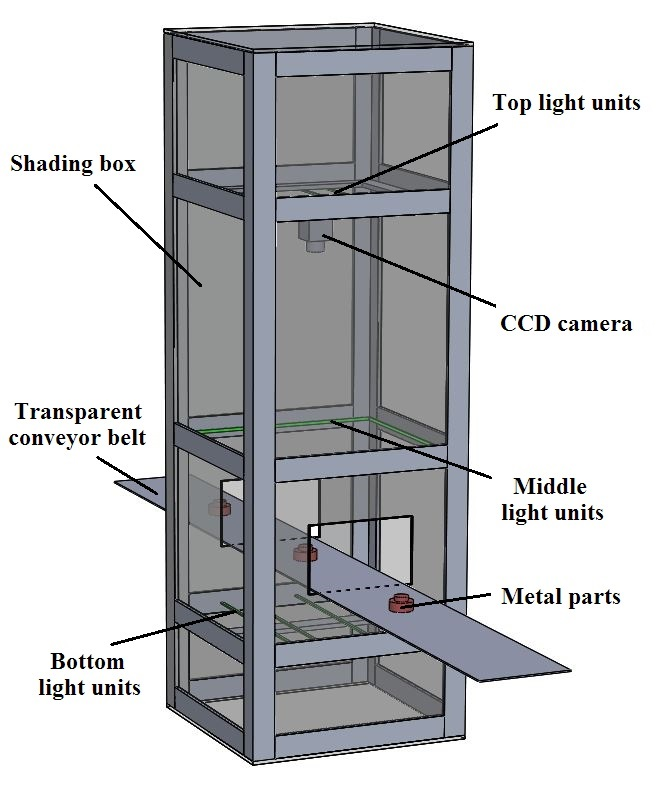
\includegraphics[width=0.8\textwidth]{figures/zheguangmokuai.png}
\caption{设备结构图}\label{zheguangmokuai}
\end{figure}
\begin{enumerate}
\item 遮光模块:为了捕捉特定入射角度光源下的照片,我们需要提供一个屏蔽其它光源的拍摄环境,为此我们将整个设备设计在一个合适大小$(60cm\times 60cm\times 110cm)$的遮光箱(如图\ref{zheguangmokuai}内标记Shading box 部分)内。为了整个设备的稳固和耐用,遮光箱用金属材质搭建框架,并在框架上面覆盖了黑色塑料板,形成一个密闭的环境。同时,为了避免遮光箱本身材质对光的反射,影响灯光环境,我们使用一种黑绒布材料覆盖在遮光箱内部,该材料具有吸光的特性,能削弱遮光箱本身材质对光照环境的影响。
\item
平台模块:由一块固定在距遮光箱底部
$10cm$处的一个白色亚力克匀光板组成,用来放置需要扫描的零件,
在应用到零件生产流水线上时,可以用一个传送带(图\ref{zheguangmokuai}中Transparent conveyor belt)替代。
该匀光板放置物体的一面为磨砂面,反射效果较弱,可以削弱对入射光的反射,减小对光照环境的影响。
\item
灯光模块:该模块为拍摄提供特定的灯光环境,环境要求灯光为满足一定入射角度的平行光源,
同时尽可能的避免散射和衰减。此模块包括周围四组光源(图\ref{zheguangmokuai}中Middle light units)、顶部光源(图\ref{zheguangmokuai}中Top light units)以及覆盖在光源上的的CPL滤光膜。所有的光源均由一组LED灯带组成,既保证了光源质量,又节约了成本。
周围四组光源设置在平台模块上$20cm$处的遮光箱四壁,
通过一个金属槽卡住LED灯带,分别从放置物体平台的前(东)、后(西)、左(南)、右(北)
四个方向以${45}^{\circ}$角照射平台中央。拍摄时,当东部灯组亮起,零件照片呈现出上半部分较亮,下半部分较暗的特点,西部灯光组亮起则与之相反;南部灯组亮起,捕获的照片左半部分会较亮,右半部分较暗,北部灯组亮起来时呈相反特点。顶部灯组由四条LED灯带组成,固定在相机镜头下$3cm$处,垂直照向平台中心。CPL滤光膜具有选择性通过某个方向光线的功能,配合数码相机的偏光镜头能起到滤除高光的作用。我们在所有的灯带上均放置了滤光膜,搭配相机的偏光镜使用,滤除金属零件表面高光。
\item
拍照模块:拍照模块包括一款单反相机和偏光镜镜头。本文所用相机为Nikon D9000。相机固定于遮光箱顶部正中间位置,使镜头正对着平台正中心。在镜头下方放置一个偏光镜头,通过步进电机控制其位置,电机正向转动,可将偏光镜移到镜头下方,反向转动,可将偏光镜移开。
\item
控制模块:控制模块由单片机、继电器、步进电机和他们的配套驱动、电源组成。单片机分别于继电器和步进电机相连,用来控制继电器的开闭和步进电机的转、停、换向。继电器连在灯光线路上,被当做光源的开关,它的开闭代表着电路的通断,步进电机被用来控制偏光镜的位置。通过这种设计,
单片机输出不同的高低电平即可控制灯光的开闭和偏光镜的位置,而我们只需要将计算机连接到单片机上,通过控制单片机即可实现整个硬件设备的控制。
\end{enumerate}

完成所有模块的设计之后,通过这一设备即可对零件进行扫描,获取
拍照结果,其结果如图
\ref{caputure}
所示。
图\ref{caputure}中图组$(a)$
为使用了偏光镜和滤光膜滤除了高光之后的拍照结果,
图组$(b)$
为保留了高光得到的拍照结果。
图组$(a)$中
$North$表示北部灯光组亮起时的拍照结果,此时照片上半部分较亮,下半部分较暗,
记为$Image\_N1$;
$South$表示南部灯光组亮起时的拍照结果,此时照片下半部分较亮,上半部分较暗,
记为$Image\_S1$;
$West$表示西部灯光组亮起时的拍照结果,此时照片左半部分较亮,右半部分较暗,
记为$Image\_W1$;
$East$表示东部灯光组亮起时的拍照结果,此时照片右半部分较亮,左半部分较暗,
记为$Image\_E1$;
$Top$表示顶部灯光组亮起时的拍照结果,记为
$Image\_T1$。
保留高光时,
对应的图片分别记为$Image\_N2$、$Image\_S2$、$Image\_W2$、$Image\_E2$、$Image\_T2$。

\begin{figure}[htbp]
\centering
	\begin{minipage}[]{1.0\linewidth}
	\centerline{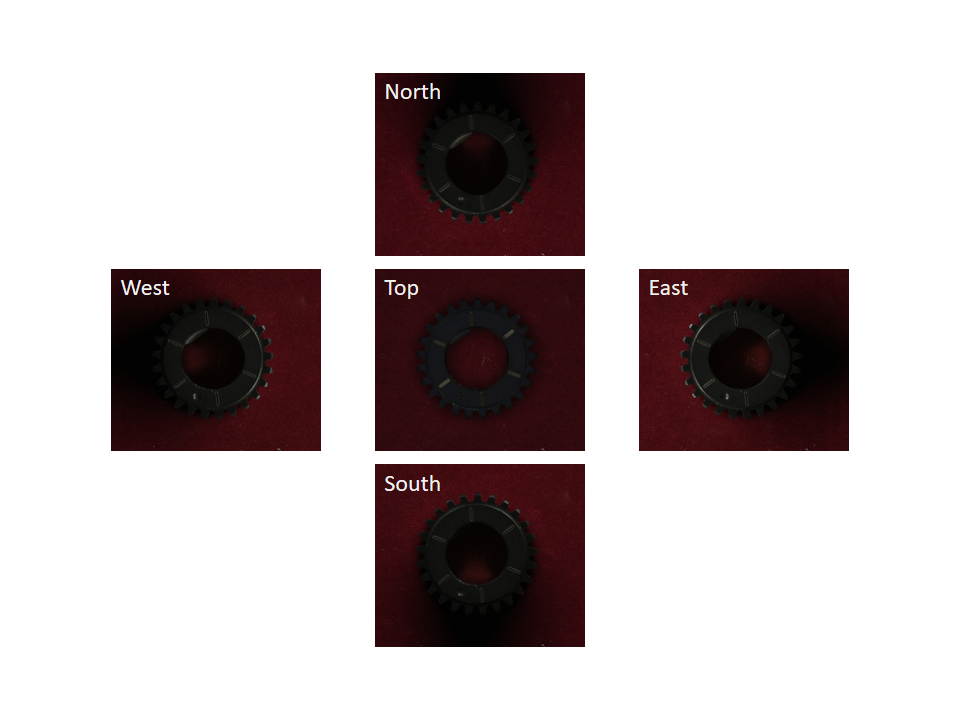
\includegraphics[width=1\linewidth]{figures/capturea.png}}
	\centerline{
		\footnotesize{(a)}}
	\label{caputurea}
	\end{minipage}
	\begin{minipage}[]{1.0\linewidth}
	\vspace{-1pt}
	\centerline{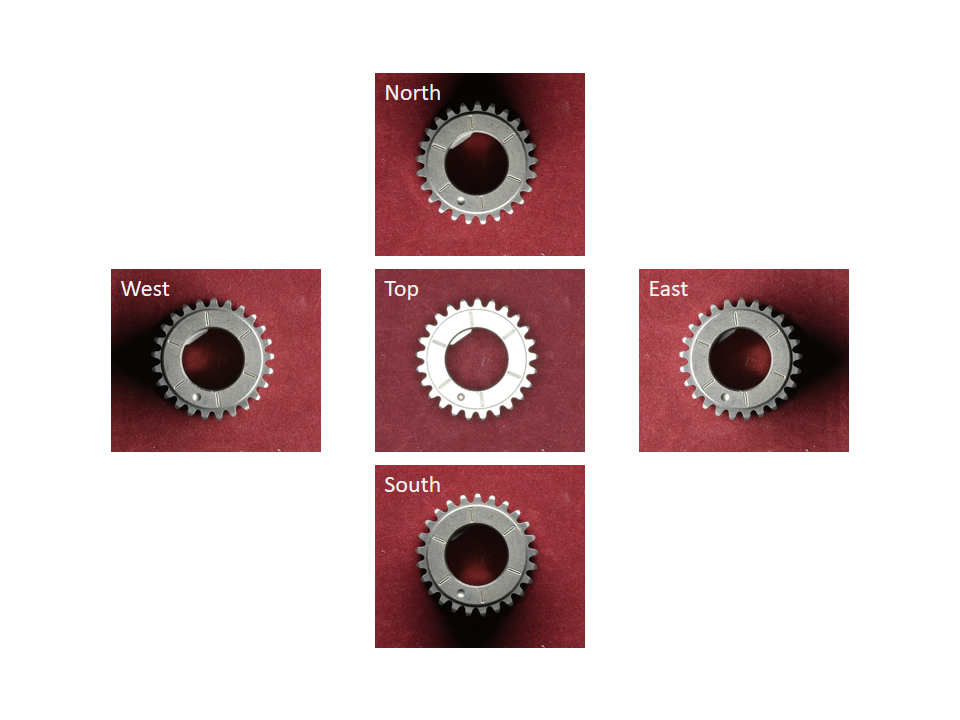
\includegraphics[width=1\linewidth]{figures/captureb.png}}
	\centerline{
		\footnotesize{(b)}
	}
	\label{caputureb}
	\end{minipage}
\caption{扫描结果:(a)表示滤除高光的结果,(b)表示保留高光的结果}
\label{caputure}
\vspace{-5pt}
\end{figure}

\section{算法设计与实现}

本节介绍提取零件表面法线的算法。该算法使用上节设备得到的零件照片作为输入,基于光线的反射原理计算零件表面
法线。同
时,为了优化照片的质量,提高零件法线的精度,本节首先对相机进行了
校正,这些校正包括白平衡校正、色彩校正、畸变校正;接着对方向光源
产生的损失进行了光线补偿,该补偿算法预存储了一套补偿数据,并利用
预存储的补偿数据对新的照片进行光线补偿;最后详细描述法线计算方法。
值得一提的是,我们的法线
提取算法不仅可以用来获取零件法线,也可以用来获取其他物体的法线。

\subsection{白平衡校正}

白平衡校正指在图像处理过程中,对原本为白色的物体进行色彩还原,使其在图片中也是白色,从而去除光源色温的影响。本文中白平衡校正用来去除LED灯带的色温。
白平衡校正有两个基础理论:灰度世界理论和完美反射理论。白平衡算法大都基于这两个理论,比如Xiaoqiang Li\cite{10.1007/978-3-642-37149-3_38}提出的算法就是对灰度世界算法的改进,Lam 和Edmun Y\cite{lam2005combining}将这两个理论结合,提出了一种自动白平衡算法。
本文白平衡校正算法基于Weng\cite{weng2005novel}等人提出的校正算法,
并在此基础上作出优化。该算法分为两步,首先检测白点,接着用白点调整色温。
在校正前,我们首先计算图片$YC_b C_r$颜色空间的值,
计算公式如\eqref{eq:rgb2gray}所示,其中$R$、$G$、$B$分别代表原来$RGB$
色彩空间中三个通道的值,$Y$、$C_b$、$C_r$分别代表了$YC_b C_r$空间各个通道的值。
\begin{equation}\label{eq:rgb2gray}
\begin{split}
Y=(0.256\ast R)+ (0.504\ast G)+(0.098\ast B)+16\\
C_b=-(0.148\ast R)-(0.291\ast G)+(0.439\ast B)+128\\
C_r=(0.439\ast R)-(0.368\ast G)-(0.071\ast B)+128
\end{split}
\end{equation}
在第一步中,算法定义了一个$near-white$区域,并将该区域所有像素作为白点候选,
随后通过求解一系列约束条件得到最优白点集合。
论文中的算法需要统计所有$near-white$区域,
并进行一系列复杂的变换求解约束条件,大大限制了其速度,并且约束条件以及$near-white$区域的选取都需要设定阈值,在不同情况下需要手动调整参数。本文使用白卡辅助确定白点。
在确定白点过程中,
我们首先对照片中的白卡进行定位,识别出白卡所在位置,
接着选择白卡中白色区域作为白点候选,
从白点候选中确定最优白点集合。
在确定最优白点集合时,
我们只需要排除白点候选中的离群点即可得到最终结果。
这种优化有三点好处:一是无需手动设定参数;二是大大降低了白点统计的复杂度,提高了速度;三是白卡中的白色区域为已知真实白色,要比论文中定义的$near-white$区域更准确。

确定白点之后,算法使用Von Kries模型\cite{macadam1970sources}来调整图片。该模型首先计算通道增益,通道增益$R_{gain}$,$ G_{gain}$, $B_{gain}$可以根据公式\eqref{eq:gain}计算,
\begin{equation}\label{eq:gain}
\begin{split}
R_{gain}=Y_{max}/R_{avew}\\
G_{gain}=Y_{max}/G_{avew}\\
B_{gain}=Y_{max}/B_{avew}
\end{split}
\end{equation}
其中,$R_{avew}$、$G_{avew}$、$B_{avew}$分别代表白点集$Red$、$Green$、$Blue$三个通道像素值的均值,$Y_{max}$表示整张图片的最大亮度值。
接着照片中每一个像素使用公式\eqref{eq:brithnessadjust}进行调整,
\begin{equation}\label{eq:brithnessadjust}
\begin{split}
R_{gain}=Y_{max}/R_{avew}\\
G_{gain}=Y_{max}/G_{avew}\\
B_{gain}=Y_{max}/B_{avew}
\end{split}
\end{equation}
公式中 $R$、$G$、$B$代表原图片中相应通道的像素值,$R^{'}$、$G^{'}$、$B^{'}$则代表了调整后图片对应通道的像素值。

\subsection{颜色校正}


颜色校正又称为色彩校正,是对图像的颜色进行调整,使其更接近真实色彩的过程。人类在不同光照条件下对同一色彩感知到的的结果相同,被称为色恒定性,
然而成像系统不同于人类,并不具有这一特征,它们所获图像的色彩往往受光源、物体反射率和成像系统的光谱响应函数影响。
因此相机在不同的光照条件下对同一物体拍摄得到的图像往往不同,并且跟人眼观察到的也有差异。
为了避免成像系统的色彩偏差,必须对图像进行色彩校正,以保证相机捕获的图像能够正确捕获物体本来颜色。

颜色校正目前已有大量研究工作,主要的方法有灰度直方图统计法、灰度平衡算法等,Porikli\cite{weng2005novel}使用距离矩阵和模型函数的方法来对相机的颜色进行矫正,
Jinlong Lin\cite{porikli2003inter}等人提出了一种基于边缘检测的色偏校正算法,
利用彩色图像的边缘色度来进行颜色校正,
Hao Yu、Jian Wang\cite{yu2009color}等人则选择在Lab空间对颜色进行校正。

本文颜色校正基于设备提供的单一光照环境,因此算法不需要自适应其它环境,只需要针对我们的实验环境进行校正即可。算法使用标准24色色卡辅助校正,首先将一张标准色卡放在设备不同的光源下拍摄照片,然后识别照片中的色卡,读取色卡中不同区域的像素信息,并与标准色卡区域对应的真实值对比,
得到色彩偏差曲线,根据偏差曲线进行颜色校正。

对于一块标准的24色色卡,
 每一块色卡中都包含24种色彩,分别位于24个矩形块中,拥有不同的$R$、$G$、$B$值,我们将第i种色彩的值记作$C_{org}^i$。
 标准色卡有固定的形状,
 可以使用边缘检测提取色卡照片中的直线,接着根据直线分割出不同的区域,得到色卡中不同区域的颜色值信息。
 对不同的区域i ,我们统计该区域的像素均值记为$C_{cap}^i$,显然,这里的$C_{org}^i$和$C_{cap}^i$都是三维向量,包含$RGB$通道的像素值信息。对应照片中色卡的像素值信息和其标准值,可以得到24个色彩值对,我们使用它们拟合一个函数$f(R,G,B)$,该函数的输入为照片的$R$、$G$、$B$通道值,输出为矫正后的像素值。


\subsection{畸变校正}

由于相机成像镜头固有的透镜效应,相机成像时会对真实的景象产生一种透视失真,被称为镜头畸变。随着镜头制造工艺的不断发展,人们通过不断改善镜头材质,优化光学设计,试图消除这种畸变,然而即使最先进的材质,最完善的设计,也难以完全消除畸变,必须借助镜头畸变校正算法进一步优化。

在计算机视觉领域,畸变校正算法已经发展的非常成熟,其中最成功的是张正友教授提出的张氏标定法\cite{zhang2000flexible},该方法现已被广泛应用于相机标定和畸变校正中。
Weng J,Cohen P\cite{weng1992camera}等人提出了先估计参数后迭代校正的两步校正方法,
Heikkila J 和Silven O\cite{heikkila1997four}等人则在Weng J等人算法的基础上进行扩展,
将两步扩展到四步,
使用额外的步骤补偿镜头的圆形特性引起的图像失真问题。
但是无论这些校正算法步骤如何,都需要估计相机参数。
相机参数分为内参、外参和畸变参数,
其中畸变参数是畸变校正中最重要的参数。
相机畸变参数包括径向畸变系数和切向畸变系数,
径向畸变是由于透镜本身的凹凸性质导致,光线在远离透镜中心的地方比靠近中心的地方更加弯曲;
切向畸变主要发生于成像仪被粘贴在摄像机上的时候,
这时成像透镜本身并不完全平行于成像平面。
畸变校正算法首先获取畸变系数,计算畸变系数对图像的作用矩阵,
通过对照片进行畸变作用相反的变换,得到消除畸变的矫正图像。

本文采用张氏标定法对相机标定,
算法只关注径向畸变。一般来讲,相机径向畸变较小,可以用主点(principle point)周围的泰勒级数展开的前几项进行描述,张氏标定法选择前两项来描述。
首先我们用待标定的相机拍摄多张包含棋盘格的照片,
拍摄时保证相机位置不变,每张棋盘格角度和位置各不相同,假设我们得到n张照片,接着
分别提取n张照片中棋盘格的$m$个角点,
根据相机成像原理可以得到$2mn$个等式,
对这$2mn$个等式使用最小二乘法求解,可以得到最优的径向畸变参数$k=[k_{1}$、$k_{2}]$,最后结合相机的内参和外参,进行极大似然估计得到更准确的畸变参数,将得到的参数保存起来,在需要的时候通过公式\eqref{eq:cortjibian}对照片进行畸变校正,
\begin{equation}\label{eq:cortjibian}
\begin{split}
p=p^{'}+(p^{'}-p_{0} )[k_{1} (x^{2}+y^{2} )+k_{2} (x^{2}+y^{2} )^{2} ]\\
q=q^{'}+(q^{'}-q_{0} )[k_{1} (x^{2}+y^{2} )+k_{2} (x^{2}+y^{2} )^{2} ]
\end{split}
\end{equation}
公式中,$(p,q)$代表畸变校正后的像素坐标,
$(p^{'}, q^{'})$
表示相机拍摄照片的像素坐标,
$k_{1}$、$k_{2}$表示张氏标定法中得到的相机畸变参数,
$(p_{0},q_{0})$
为主点的坐标。

\subsection{光线补偿}

虽然我们在设计硬件时充分考虑了光线的质量,
但是在拍摄时,仍然存在光线不均匀的情况,尤其是当需要拍摄的零件本身比较大时,光线损失会更加明显,严重影响法线的计算。因此我们需要对照片进行光线补偿,从而减少光线损失带来的误差。

已有的光照补偿算法如
\cite{贾灵芝2008基于自适应光线补偿的人脸检测算法,chen2006illumination,ruiz2008illumination,malassiotis2005robust,zheng2008intra,wiegand2003overview,tan2006intra,tan2007intra}中所提到的离散余弦变换、局部自适应模板匹配等从不同的角度对光照进行补偿,本文参考了这些方法,通过模板和函数方法进行光线补偿。

我们首先统计了不同颜色和不同灰度的材质在实验环境中所表现出来的光线损失情况,
结果如图\ref{fig:guangxiansunshi}所示,其中$(a)$、$(b)$、$(c)$、$(d)$分别代表了不同材质的光线损失图,从图中可以看出不同材质的光线损失程度不同,并且,往往材质亮度越低,光线损失越小,亮度越高,光线损失越大。

\begin{figure}[htbp]

\begin{minipage}{0.48\linewidth}
\centerline{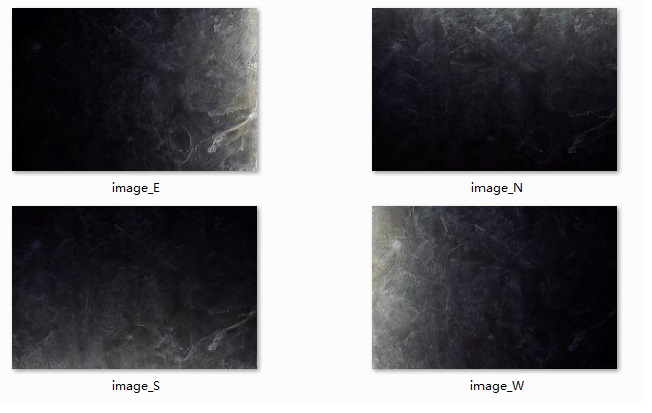
\includegraphics[width=1\linewidth]{figures/gaungxiansunshia.png}}
\centerline{(a)}
\end{minipage}
\begin{minipage}{0.48\linewidth}
\centerline{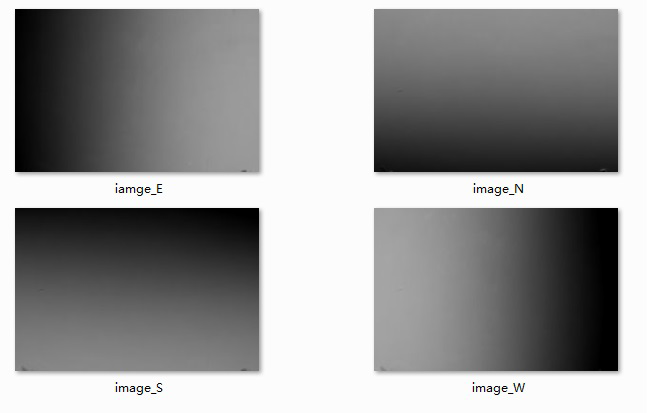
\includegraphics[width=1\linewidth]{figures/gaungxiansunshib.png}}
\centerline{(b)}
\end{minipage}


\begin{minipage}{0.48\linewidth}
\centerline{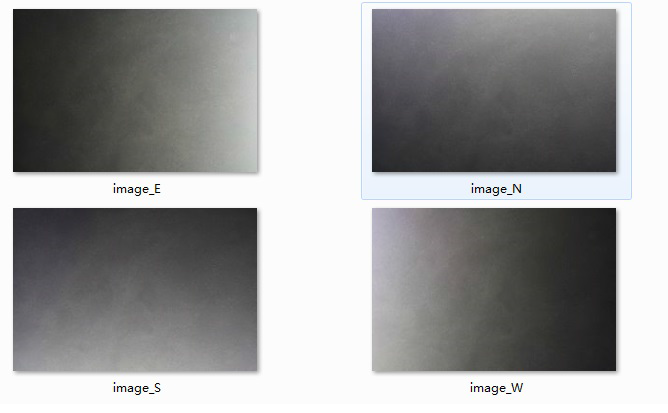
\includegraphics[width=1\linewidth]{figures/gaungxiansunshic.png}}
\centerline{(c)}
\end{minipage}
\begin{minipage}{0.48\linewidth}
\centerline{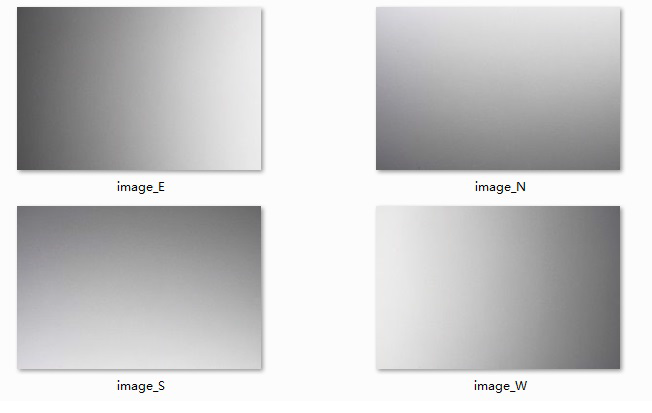
\includegraphics[width=1\linewidth]{figures/gaungxiansunshid.png}}
\centerline{(d)}
\end{minipage}

\caption{不同材质光线损失图}
\label{fig:guangxiansunshi}
\vspace{-3mm}
\end{figure}
{}
为了直观的展现光线损失和光源方向的关系,我们分别统计了照片在平行光源方向上的的衰减情况和垂直光源方向上的衰减情况,结果分别如图\ref{fig:guangxiansunshipingxing}和图\ref{fig:guangxiansunshichuizhi}所示,图中横轴表示统计方向上的位置,纵轴表示该位置上的亮度统计值,
图中不同颜色的曲线$(a)$、$(b)$、$(c)$、$(d)$分别代表了不同材质的损失曲线,
这些材质正是图\ref{fig:guangxiansunshi}中对应的材质,
$(E)$、$(W)$、$(N)$、$(S)$分别代表了东、西、北、南四个方向光源下的结果。
从图中可以明显看出,光线衰减在垂直光源方向上非常弱,但在平行光源方向上极为明显,并呈现出一种线性衰减的趋势。

\begin{figure}[htbp]

\begin{minipage}{0.48\linewidth}
\centerline{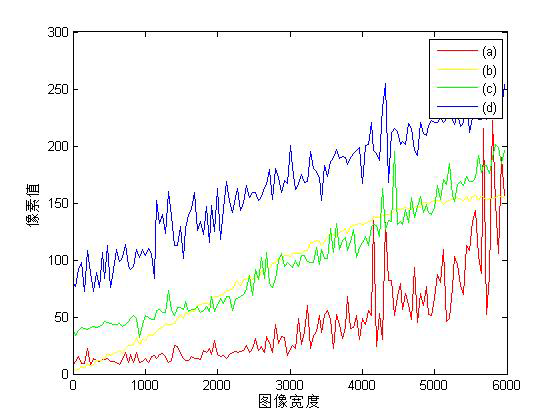
\includegraphics[width=1\linewidth]{figures/guangxianshuaijianduibituchuzhie.png}}
\centerline{(E)}
\end{minipage}
\begin{minipage}{0.48\linewidth}
\centerline{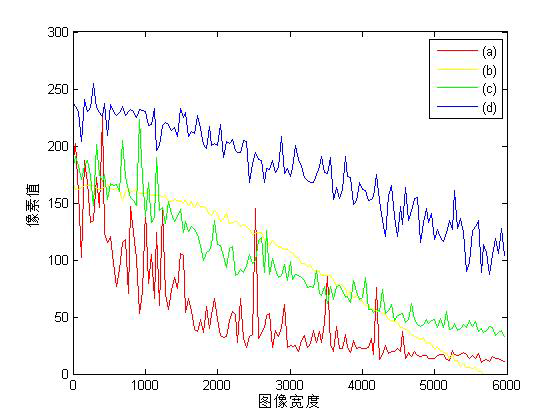
\includegraphics[width=1\linewidth]{figures/guangxianshuaijianduibituchuzhiw.png}}
\centerline{(W)}
\end{minipage}


\begin{minipage}{0.48\linewidth}
\centerline{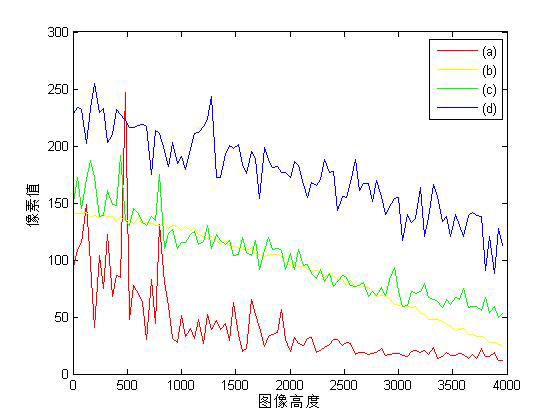
\includegraphics[width=1\linewidth]{figures/guangxianshuaijianduibituchuzhin.png}}
\centerline{(N)}
\end{minipage}
\begin{minipage}{0.48\linewidth}
\centerline{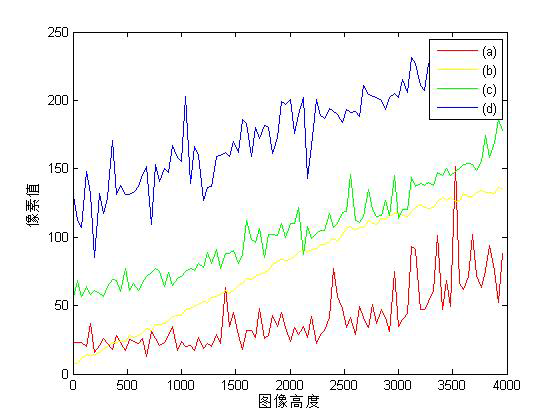
\includegraphics[width=1\linewidth]{figures/guangxianshuaijianduibituchuzhis.png}}
\centerline{(S)}
\end{minipage}

\caption{光线衰减统计图(平行光源方向)}
\label{fig:guangxiansunshipingxing}
\vspace{-3mm}
\end{figure}


\begin{figure}[htbp]

\begin{minipage}{0.48\linewidth}
\centerline{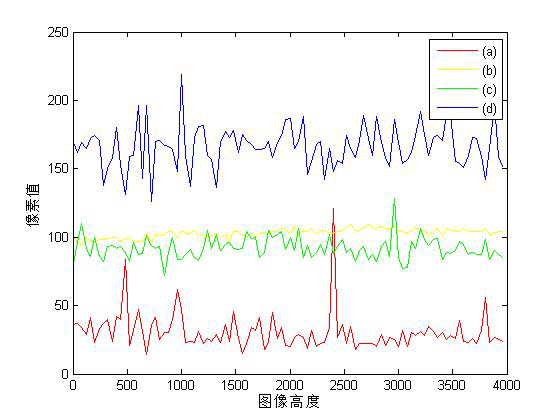
\includegraphics[width=1\linewidth]{figures/guangxianshuaijianduibitushuipinge.png}}
\centerline{(E)}
\end{minipage}
\begin{minipage}{0.48\linewidth}
\centerline{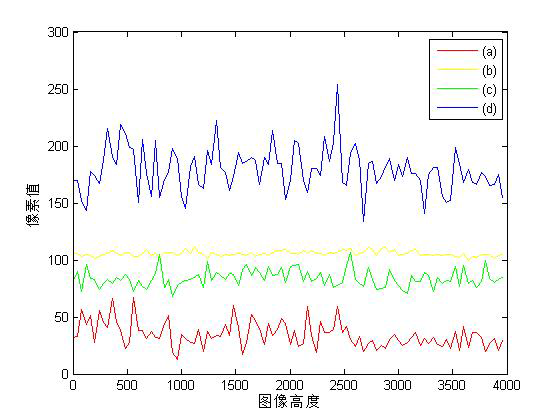
\includegraphics[width=1\linewidth]{figures/guangxianshuaijianduibitushuipingw.png}}
\centerline{(W)}
\end{minipage}


\begin{minipage}{0.48\linewidth}
\centerline{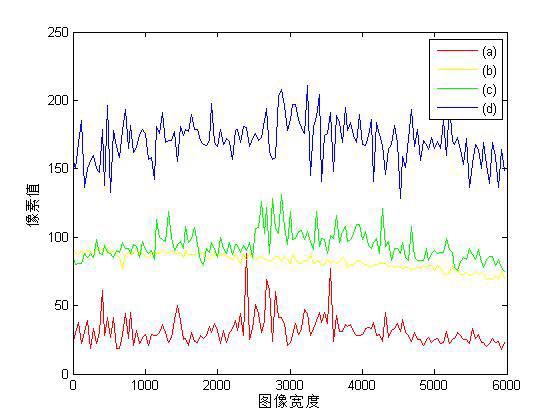
\includegraphics[width=1\linewidth]{figures/guangxianshuaijianduibitushuipings.png}}
\centerline{(N)}
\end{minipage}
\begin{minipage}{0.48\linewidth}
\centerline{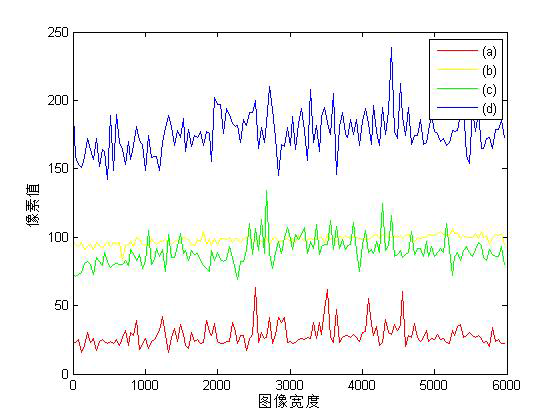
\includegraphics[width=1\linewidth]{figures/guangxianshuaijianduibitushuipingn.png}}
\centerline{(S)}
\end{minipage}

\caption{光线衰减统计图(垂直光源方向)}
\label{fig:guangxiansunshichuizhi}
\vspace{-3mm}
\end{figure}

在我们的实验环境中,相机和光源均固定不变,因此,我们可以在扫描材质前先计算一组光照补偿模板,然后针对不同的材质作出适当调整进行光线补偿。
因为我们只需对光线信息进行调整,并不涉及照片的色彩信息,
所以我们直接在亮度上进行计算,并且模板中也只保留亮度信息。
图像的亮度有多种表示方法,为了和其它步骤统一,我们使用$YC_b C_r$空间中的
$Y$分量代表亮度。

我们首先拍摄一组用来计算补偿模板的照片,这时相机直接拍摄匀光板,匀光板具有良好的光源分散性质,不容易造成光线损失。拍摄时,我们首先拍摄顶部光源下的照片,并将其作为没有损失的照片,记为
$Base$,
之后依次拍摄东部灯光组、西部灯光组、南部灯光组和北部灯光组下的待校正照片,
分别标记为${Adjust}_E$、${Adjust}_W$、${Adjust}_S$、${Adjust}_N$,
为了方便计算和节省存储空间,我们只保留他们的亮度值,
分别记为${Base}^L$、${Adjust}_E^L$、${Adjust}_W^L$、${Adjust}_S^L$、${Adjust}_N^L$。
接着我们使用${Base}^L$减去各个方向上的亮度值,得到不同方向光源上相对于Base的光线衰减信息,
为了保证补偿信息的非负性,我们为整体亮度增加一个偏差$\alpha$,
偏差的的小为${Base}^L$与${Adjust}_E^L$、${Adjust}_W^L$、${Adjust}_S^L$、${Adjust}_N^L$对应差值最小的$0.1\%$的均值。
如果结果仍为负0,我们直接将其置为0,认为此处没有损失,
最终补偿计算方法如公式\eqref{eq:guangxianbuchang}所示,
\begin{equation}\label{eq:guangxianbuchang}
{Comp}_d=\max ({0,{Base}^L-{Adjust}_d^L+\alpha }),\quad d\in \{E,W,S,N \}
\end{equation}
其中${Comp}_d$表示对应方向光源下的补偿信息,$\alpha$表示偏差,计算方法如公式\eqref{eq:paincahzhijisuan}所示,
其中$NMIN$表示集合对应差值的最小的$N_{min}$个值的集合,$N_{min}=N\times 0.001$,N表示图片的像素值总数。
\begin{equation}\label{eq:paincahzhijisuan}
\alpha =\frac {1}{N_{min}} \sum_{i}^{N_{min}}{Y_i},\quad Y_i\in NMIN
\end{equation}

考虑到不同亮度材质的光线损失程度不同,我们在校正时会对模板信息做相应调整。
根据前面的统计规律,我们使用线性函数对模板进行调整。当需要进行光线补偿时,记不同方向光源下的照片为
${Image}_d$,其中$d \in \{E,W,S,N\}$,
在顶部光源下拍摄的照片为${Image}_T$,我们用公式\eqref{eq:guangxianbuchangsuanfa}计算对应的补偿,
\begin{equation}
\label{eq:guangxianbuchangsuanfa}
{CImage}_d^L={Image}_d^L+\lambda*{Comp}_d*(avg({Image}_T^L)/avg({Base}^L))
\end{equation}
其中avg表示求平均值函数,${Image}_d^L$表示不同方向光源下照片的亮度值,
${CImage}_d^L$表示光线补偿后照片的亮度值,
$\lambda$为补偿强度参数,表示光线补偿的强度,
本文实验$\lambda$取$0.8$,如果需要增大补偿强度,可以将其调高。

\subsection{法线计算}


 Ryan Clark\cite{zarria.net}提出了一种在没有光线损失情况下的计算方法,
 他使用photoshop工具模拟了算法,并没有将该算法系统化,算法所得到的法线信息在细节和整体上都存在极大问题。
 并且,算法没有考虑光线损失对结果的影响。
 本文受该算法启发,利用光照反射原理计算法线,不仅此基础上增加了对光线损失的补偿,而且利用不同方向光源下的照片来计算,取得了更好地结果。

\begin{figure}[htbp]
\centering
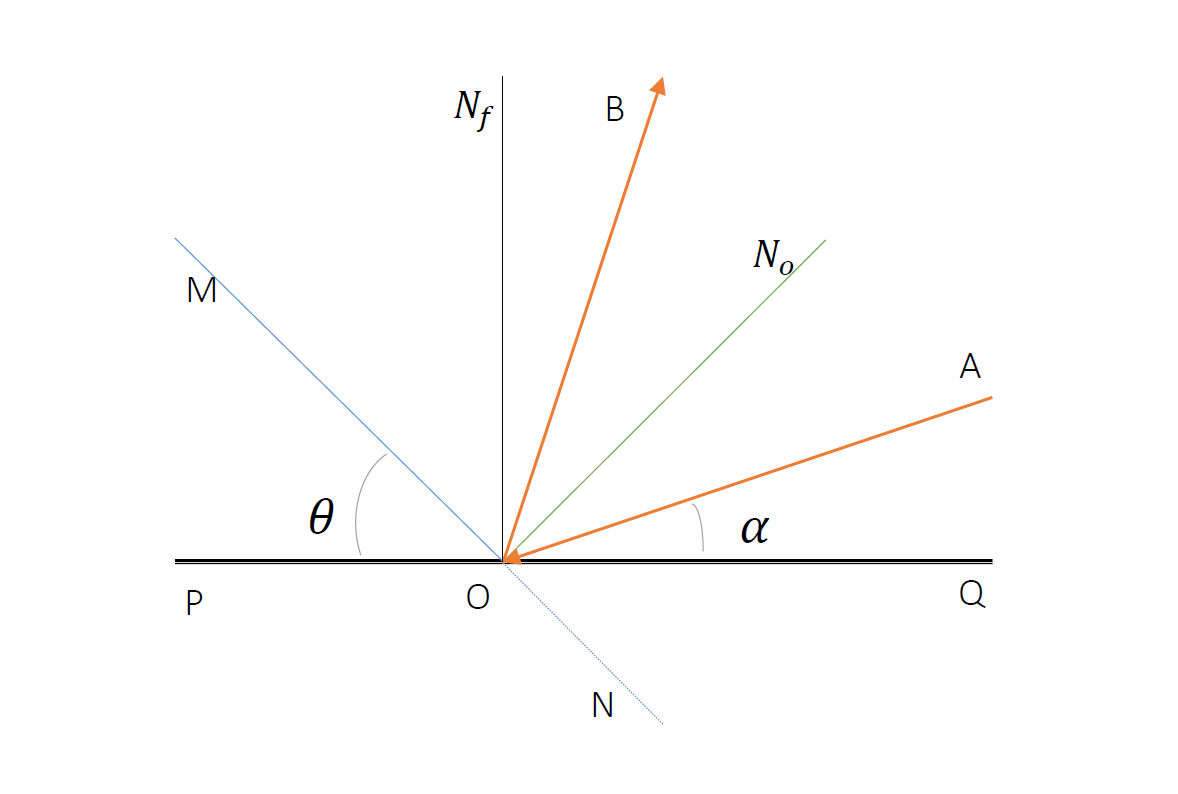
\includegraphics[width=1.0\linewidth]{figures/guangxianfanshetu.png}
\caption{光线反射原理图}
\label{fig:guangxianfanshetu}
\end{figure}

光照反射原理如图\ref{fig:guangxianfanshetu}所示,其中$PQ$表示水平面,
$MN$表示物体表面,
实线部分$MO$
为真实表面,
$ON$
是表面的延长,是为了方便观察和理解,
$\overrightarrow{AO}$为入射光,
$\overrightarrow{OB}$表示反射光,
$ON_f$
表示水平面的法线,垂直于
$PQ$,
$ON_o$表示物体表面法线,
垂直于$MN$,
$\angle POM$
为物体表面和水平面的夹角,记为
$\theta $,
$\angle AOQ$为入射光与水平面的夹角,记为
$\alpha$。在本系统中,实验环境固定,
相机镜头平行于水平面$PQ$,
不同方向光源和水平面的夹角为
$45^{\circ}$,
因此$\alpha=45^{\circ}$。
假设入射光线的强度为$I$,由
$\angle POM=\theta$和
$\angle AOQ=\alpha$易得
$\angle {BON}_f=2\theta+\alpha-90$
。根据光的反射原理,在不考虑其他介质对光的散射时,
反射到相机中的光线强度可以用公式\eqref{eq:guangxianqiangdu}来计算,
\begin{equation}
\label{eq:guangxianqiangdu}
I_{ref}=\lambda I* \cos (2\theta +\alpha-90)
\end{equation}
其中,$\lambda$表示光线反射率,
当光源相同时,光线反射率不变,
$\alpha$已知,为
$45^{\circ}$,
根据公式\eqref{eq:guangxianqiangdu},理论上反射到相机中的光照强度只有材质表面的倾斜角度有关,
光照强度反应在拍摄图片的亮度信息中,
因此拍摄照片的亮度信息必然只与材质本身的倾斜角度有关,
即亮度信息只和材质的法线有关,
根据这一推论,
我们可以使用四个不同方向光源下的照片来计算物体的法线。

我们首先获取不同方向光源下的照片
$Image\_E1$、$Image\_W1$、$Image\_N1$、$Image\_S1$,
使用光线补偿算法对其进行光线补偿,并得到其亮度信息,
记为
${Image}_E^L$、${Image}_W^L$、${Image}_N^L$、${Image}_S^L$,
接着我们创建两个新的三通道图
$NorthWest$和$SouthEast$
用来保存数据,其中
$NorthWest$的$R$通道保存
${Image}_W^L$,
$G$通道保存
${Image}_S^L$,
$SouthEast$的$R$通道保存
${Image}_E^L$,
$G$通道保存
${Image}_S^L$,
接着我们将$NorthEast$的色阶调整到$[0.0-0.5]$,
将SouthEast的色阶调整到$[0.5-1.0]$,
调整色阶的计算方法如公式\eqref{eq:tiaozhengsejie}所示,
其中$p$表示图像的像素值,
$a$为调整后色阶的上界,$b$为调整后色阶的下界,${p}^{'}$为调整后的像素值。
\begin{equation}
\label{eq:tiaozhengsejie}
{p}^{'}=p* (a-b)+b
\end{equation}
最后我们将$NorthWest$
和$SouthEast$叠加成一张法线图$Normal\_Temp1$,
叠加时使用公式
\eqref{eq:hunhetuxiang}
计算。
\begin{equation}
\label{eq:hunhetuxiang}
Normal\_Temp1=2* NorthWest* SouthEast
\end{equation}
这一法线图中包含了$R$和$G$通道的信息,由法线的归一化性质,我们可以根据R和G通道的值来计算B通道的值,计算方法如公式\eqref{eq:btongdaojisuan}所示,
其中$r$表示R通道像素值,$g$表示$G$通道的像素值,$b$表示$B$通道的像素值。
\begin{equation}
\label{eq:btongdaojisuan}
b=2.0* \sqrt{1.0-{(r-0.5)}^2+{(g-0.5)}^2}-1.0
\end{equation}

我们将$Image\_N2$、$Image\_S2$、$Image\_W2$、$Image\_N2$也使用上述处理方式,
可以得到有高光情况下的法线图$Normal\_Temp2$。
$Normal\_Temp1$滤除了高光,光线信息较弱,
细节部分表现较弱,但是整体结果较好,
$Normal\_Temp2$保留了高光信息,光线信息较强,细节表现明显,但部分区域容易出现法线的跳跃现象,因此我们使用alpha融合算法融合这两张法线图,得到最终法线,融合方法如公式
\eqref{eq:faxianronghe}所示。
\begin{equation}
\label{eq:faxianronghe}
Normal=(Normal\_Temp1+Normal\_Temp2)* 0.5
\end{equation}

实验结果如图\ref{fig:faxianjieguotu}所示,
其中$(a)$表示零件原图,$(b)$表示算法得到法线图,
我们的法线图既保留了细节信息又不会出现法线跳跃现象,具有良好的性质。

\begin{figure}[htbp]
\centering
\begin{minipage}{0.48\linewidth}
\centerline{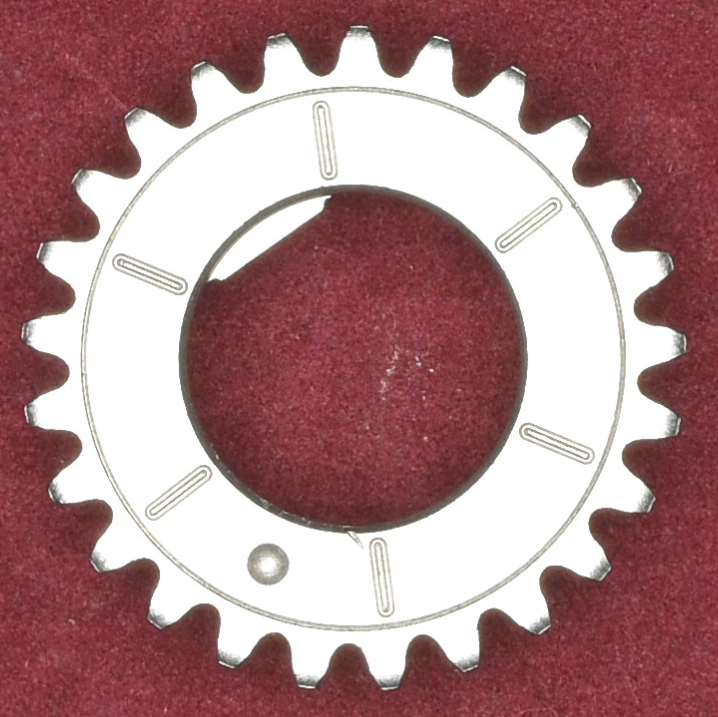
\includegraphics[width=1.0\linewidth]{figures/faxiantuyuantu.png}}
\centerline{(a)}
\end{minipage}
\begin{minipage}{0.48\linewidth}
\centerline{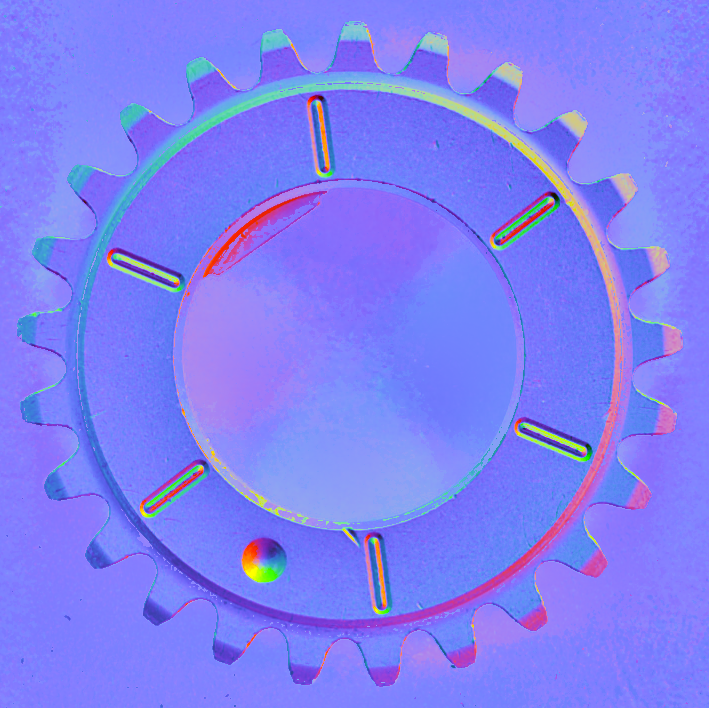
\includegraphics[width=1.0\linewidth]{figures/faxiantujieguo.png}}
\centerline{(b)}
\end{minipage}
\caption{法线提取结果图}
\label{fig:faxianjieguotu}
\end{figure}

\section{实验结果}

本节首先介绍我们的硬件设备成品,接着介绍法线提取结果并与其他相关工作对比。
由于本章设计的法线提取算法不仅可以用于提取零件表面法线,还可以被扩展到任意材质的法线提取中,因此我们将它独立成一个模块,用于提取材质法线图,本节不仅包含零件表面法线提取结果,还包含了对其它材质的法线提取结果。

\subsection{硬件设备结果}

遵循\ref{section:yingjianshebeidesheji}节中的硬件设计,
我们给出了实现,并将其应用到了实际生产中。
设备由5个模块组成,这些模块被封装到一个白色的铝合金外壳中,如图\ref{fig:yingjianjieguo}所示,
$(a)$展示了设备的整体外观,
为了移动方便我们在设备底部安装了四个滚轮,
设备顶部可以打开,
如
图\ref{fig:yingjianjieguo}中$(b)$所示,打开之后可以看到固定在顶部的相机、滤光镜和顶部灯光组,
图\ref{fig:yingjianjieguo}中$(c)$展示了更清楚的结果,
设备中间部分如
图\ref{fig:yingjianjieguo}中$(a)$所示,
保留了一个门,门内
如$(d)$和$(e)$
所示,可以看到摆放材质的平台和不同方向的灯光组,
需要扫描的材质放在这个平台中间,灯光组以
${45}^{\circ}$
照向平台中间,从
图\ref{fig:yingjianjieguo}中$(b)$、$(c)$、$(d)$、$(e)$中都可以看到内部的黑色绒布,
这些绒布有吸光性质,可以减少了对光照的影响。

\begin{figure}[htbp]
\centering
\centerline{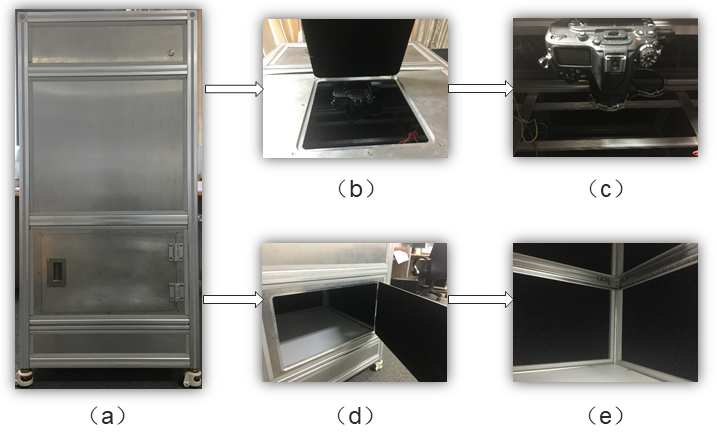
\includegraphics[width=1.0\linewidth]{figures/yingjianjieguo.png}}
\caption{硬件示意图}
\label{fig:yingjianjieguo}
\end{figure}

\subsection{法线提取结果}

在计算法线之前,我们先对相机进行白平衡校正、颜色校正、畸变校正以及光线补偿,保存它们的参数,用来对之后拍摄的照片校正。随着时间的推移,不论是相机还是光源都会有细微的变化,
为了保证参数的准确性,
在实际应用中我们定期的对相机进行这些校正,
更新校正参数。经验表明,至少三个月需要对设备重新校正一次。

获得校正参数之后,我们首先使用设备拍摄不同光源下的零件照片,
接着运行校正算法,最后计算零件表面法线。
为了拍摄不同光源下的零件照片,我们首先将目标放置在设备的平台中央,
接着使用程序控制硬件设备获取所需照片。
获取的过程分为两步,
第一步相机使用滤光镜,
程序分别控制亮起顶部灯光组、东部灯光组、西部灯光组、北部灯光组、南部灯光组并拍摄照片,并对照片进行校正,
保存结果为$Image\_T1$、$Image\_E1$、$Image\_W1$、$Image\_N1$、$Image\_S1$;
第二步中程序控制电机转动移开滤光镜,重复第一步中的步骤,对零件拍照和校正,
并存储结果为$Image\_T2$、$Image\_E2$、$Image\_W2$、$Image\_N2$、$Image\_S2$。
最后,使用这些数据运行法线提取算法,即可得到零件法线,
法线图结果如图\ref{fig:faxianjieguotu}所示。

在材质表面信息获取领域中,Vizoo3D xTex开始最早, 
并仍保持着业界领先水平,我们将本文结果与其结果作对比。
\begin{figure}[htbp]
\begin{minipage}{0.48\linewidth}
\centerline{
\includegraphics[width=1.0\linewidth]{figures/faxianduibia.png}}
\centerline{(a) Vizoo3D xTex的结果图 }
\end{minipage}
\begin{minipage}{0.48\linewidth}
\centerline{
\includegraphics[width=1.0\linewidth]{figures/faxianduibib.png}}
\centerline{(b) 本文结果图}
\end{minipage}
\caption{法线结果对比图}
\label{fig:faxianjieguoduibi}
\end{figure}
我们首先得到他们对某一材质的法线提取结果,
然后使用我们拥有的最相似的材质提取法线并对比,结果如图\ref{fig:faxianjieguoduibi}
所示,其中
$(a)$表示Vizoo3D xTex得到的法线结果,
$(b)$为我们提取的法线结果,从图中可以看出这组法线都比较平整,
不存在褶皱等问题,
但是
$(a)$中的法线信息在中心处要比边缘部分模糊,
我们推测这可能是由于光线不均或光线损失导致,
而我们在法线计算过程中考虑了这一问题,因此我们的结果可以在不同区域保持一致。
图\ref{fig:faxianjieguotu}中展示了我们提取的其他材质的法线图,
其中$(a)$、$(b)$、$(c)$、$(d)$分别代表了不同材质的法线图,
从图中可以看出,对于不同的材质我们都能够得到较好的法线提取结果。
\begin{figure}[htbp]
\begin{minipage}{0.48\linewidth}
\centerline{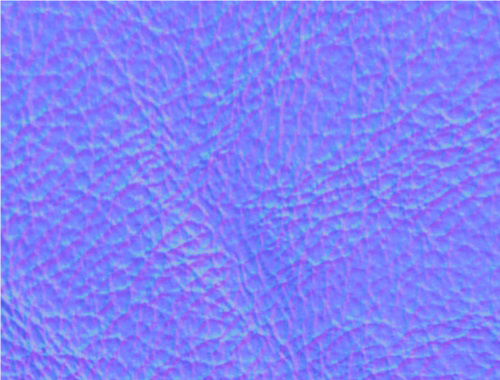
\includegraphics[width=1.0\linewidth]{figures/faxianjieguotua.png}}
\centerline{(a)}
\end{minipage}
\begin{minipage}{0.48\linewidth}
\centerline{
\includegraphics[width=1.0\linewidth]{figures/faxianjieguotub.png}}
\centerline{(b)}
\end{minipage}

\begin{minipage}{0.48\linewidth}
\centerline{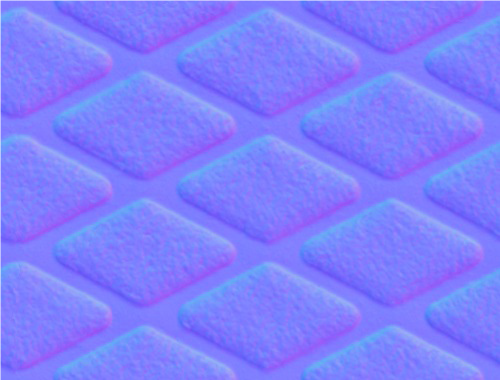
\includegraphics[width=1.0\linewidth]{figures/faxianjieguotuc.png}}
\centerline{(c)}
\end{minipage}
\begin{minipage}{0.48\linewidth}
\centerline{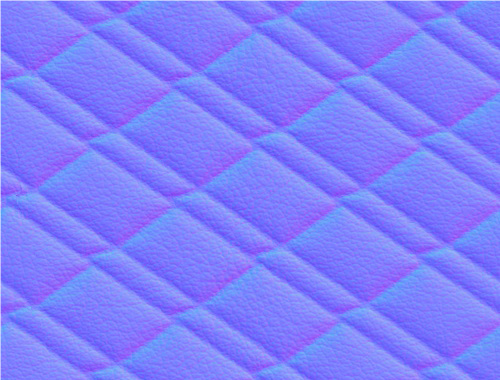
\includegraphics[width=1.0\linewidth]{figures/faxianjieguotud.png}}
\centerline{(d)}
\end{minipage}

\caption{法线结果图}
\label{fig:faxianjieguotu2}
\end{figure}

%传统方法
\chapter{基于传统算法的缺陷检测}
\label{chapter:chuantongfangfa}

基于传统算法的缺陷检测一般由获取原始图像、数据预处理、特征提取、训练分类器、使用分类器得到检测结果这几个步骤构成,
本章算法基于以上步骤,对每个环节做了相应优化。
其中,获取原始图像中我们使用上一章介绍的方法获取零件法线图,我们不再过多介绍。
本章首先介绍如何对数据进行预处理,接着介绍如何设计和提取图像特征,
之后介绍本文使用的分类器模型,
最后介绍如何对模型训练和分类,并给出实验结果和分析。

\section{数据预处理}

往往数据和特征决定了机器学习的上限,模型和算法仅仅用来逼近这个上限,
因此数据预处理是算法中非常重要的部分。
在数据预处理之前,我们首先利用前一章中的算法获取零件表面法线,获取法线的过程本身也是对相机照片的一种处理。
接着本文将获零件法线图用于缺陷检测,
由于零件大多呈环状,在得到的法线图中,背景占比过大,因此我们首先设法去除背景,提取零件的主要表面进行缺陷检测。
在生产过程中零件缺陷的出现概率很小,
限制了数据的规模,针对这一问题,我们用数据增强的方法来增加样本数量,扩充数据库。

\subsection{零件主表面获取}

一方面,法线图中零件表面所占比例过低,背景较多,严重影响了算法的性能和表现,
另一方面,零件生产过程中,边缘部分不容易产生缺陷,并且其缺陷也容易检测,
因此,本节提取零件主要非边缘部分,称为主表面,
之后针对主表面做数据增强。
在工业生产中,零件的设计是有一定规则要求的,
因此零件往往非常相似,
本节针对一种零件设计提取算法,
该算法能够简单地推广到相似的零件中。
在获取不同光源下照片的过程中,相机位置和零件位置都是不变的,
因此对于同一组零件照片,
我们只需要在一张图片中提取出主表面即可获得所有照片和法线图的主表面,
本节使用$Image\_T 2$提取主表面。

首先,使用
公式\eqref{eq:huiduzhuanhuangognshi}
将$Image\_T 2$转化为灰度图,
其中,$Gray$表示转化结果,
$R$、$G$、$B$表示输入图片$RGB$色彩空间中对应通道的值。
\begin{equation}
\label{eq:huiduzhuanhuangognshi}
Gray=R*0.299+G*0.587+B*0.114
\end{equation}
接着我们将灰度图二值化,
二值化分两步,首先使用最大类间方差来确定一个阈值
$b\_t$,
然后将所有大于该阈值的像素值设为1,小于或等于该阈值的值设为0,即可得到二值图像。
\begin{figure}[htbp]
\centering
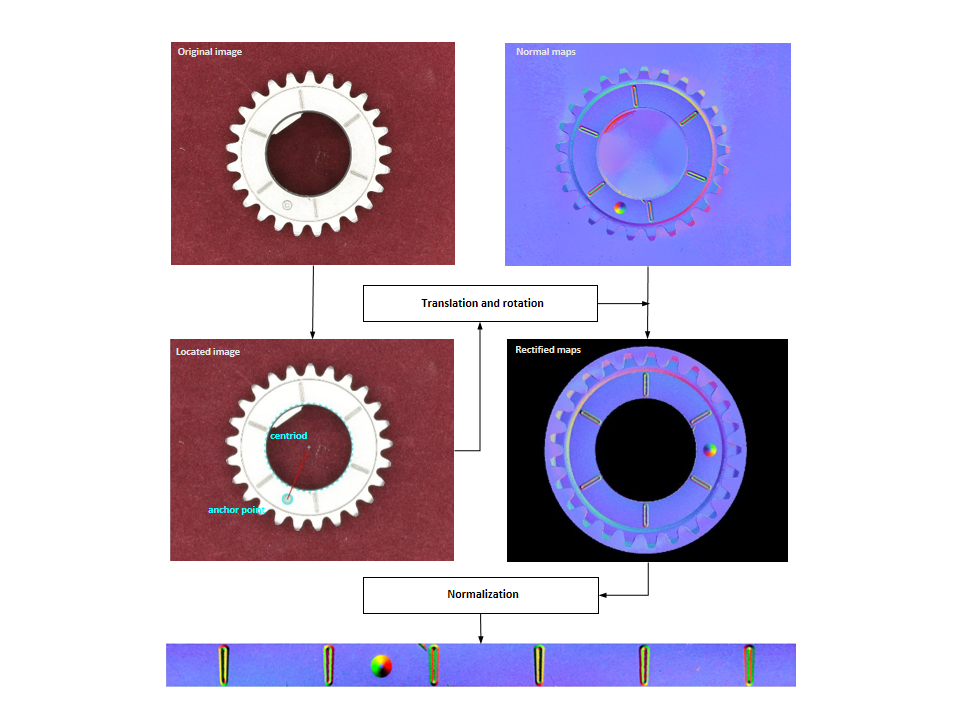
\includegraphics[width=1.0\linewidth]{figures/jiaozhengliuchengtu.png}
\caption{主表面获取结果图}
\label{fig:zhubiaomianhuoquliucheng}
\end{figure}

最大类间方差法又叫做大津法,
该方法假设阈值为${t}^{'}$,
使用${t}^{'}$将图片分为前景(值为1)和背景(值为0)两个区域,
其中属于前景的像素点占图像的比例记为${w}_{0}$,平均灰度值信息记为${u}_{0}$,
背景像素点占图像的比例记为${w}_{1}$,
平均灰度值记为${u}_{1}$,
图像的大小记为
$M\times N$,平均灰度值记为$u$,
类间方差记为$g$,
图像中小于阈值${t}^{'}$
的像素个数记为
${n}_{0}$,大于
${t}^{'}$的像素个数记为
${n}_{1}$,
于是我们可以得到等式\ref{fig:jisuanw0}、\ref{fig:jisuanw1}、\ref{fig:jisuang}。
\begin{gather}
{w}_{0}={n}_{0}/(M\times N) \label{fig:jisuanw0}\\
{w}_{1}={n}_{1}/(M\times N)\label{fig:jisuanw1}\\
g={w}_{0} {({u}_{0}-u)}^{2}+{w}_{1}{(u_1-u)}^{2} \label{fig:jisuang}
\end{gather}
因为灰度值的范围为
$[0-255]$,我们可以使用遍历的方法找到使
$g$最大的
${t}^{'}$,
把这个值作为阈值$b\_t$。

接着我们对生成的二值图像做腐蚀操作,
并去除一些小的连通区域,
然后对其进行膨胀操作,
得到零件和背景分开的二值图像。
在这个二值图像中,
背景被圆环状零件分割成两个部分,
一部分位于圆环中心,
另一部分将零件包裹,
我们首先提取圆环中心部分的质心和半径得到一个内切圆,
接着提取环状零件的圆心和半径,最后提取圆环上的圆形定位点。
结果如图\ref{fig:zhubiaomianhuoquliucheng}所示,
图中$Original image$表示零件照片,
$Normal imgae$表示零件法线图,
$Localted image$表示提取圆心和定位点的结果,
其中蓝色虚线表示提取的圆环中心圆,蓝色实线圆表示零件定位点,红色直线连接了定位点的圆心和圆环中心圆的圆心。
根据提取出来得信息,我们去除掉零件背景区域,
得到圆环状区域$Rectified maps$,
最后我们将环状区域展开成一个矩形,并裁剪掉其边缘部分,得到图\ref{fig:zhubiaomianhuoquliucheng}中最底部显示的零件主表面图。

\subsection{数据增强}
\label{subsection:shujuzengqiang}

首先,随着制造业、冶金业的高速发展,零件的制造工艺不断提高,零件生产过程中缺陷产生的概率变得很小,导致我们拥有的数据量较小,需要使用数据增强的方式扩充数据;
其次,缺陷具有一定旋转不变性,
可以在数据增强阶段体现这一性质。

\subsubsection{分割}
\label{subsubssection:chuantongfenge}

我们首先使用滑动窗口将一张主表面图分割成一组固定大小的图片,
实验过程中,滑动窗口大小固定,
用$WinSize$来表示,
划分后的图片大小和窗口大小相同。
在确定$WinSize$的大小时,
我们遵循两个原则:(1)尽可能使缺陷占图片较大比重;(2)尽可能使图片包含任意单独缺陷。
为了选择合适的$WinSize$,
我们首先人工标记了所有缺陷的
矩形包围盒,这些包围盒的大小用$(w_i,h_i)$表示,
其中$w_i$、$h_i$分别表示第i个包围盒的宽和高,
包围盒宽和高的最大值分别用${w}_{max}$、${h}_{max}$表示,
最小值用${w}_{min}$、、${h}_{min}$表示,
接着我们分别统计了宽和高的直方图,其范围分别为$[{w}_{max},{w}_{min}]$,
$[{h}_{max},{h}_{min}]$,
我们通过观察直方图,确定$WinSize$的大小。
在实验过程中,我们分别尝试过$21*21$、$25*25$、$32*32$、$40*40$
等不同尺寸的窗口,
其中$25*25$的实验效果最理想,为我们最终确定的窗口。
窗口分割结果如图\ref{fig:chuangkoufenge}所示,
$WinSize$为$25*25$,滑动窗口步长为17。
\begin{figure}[htbp]
\centering
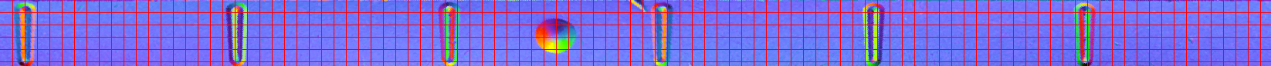
\includegraphics[width=1.0\linewidth]{figures/chuangkoufengetu.png}
\caption{滑动窗口分割示意图}
\label{fig:chuangkoufenge}
\end{figure}

\subsubsection{镜像和旋转}

对于一个有缺陷的零件图片,对其镜像和旋转之后,仍然是一个有缺陷的零件图片,在法线图上也是如此,因此我们可以使用镜像和旋转的方式扩充数据库。
经过分割之后,
所有的数据都变为$25*25$大小的图片,
我们首先对这些图片做镜像,产生新的图片,
接着将所有的图片分别顺时针旋转$45^\circ$、$90^\circ$、$135^\circ$、$180^\circ$、$225^\circ$、$270^\circ$、$315^\circ$,得到新的数据。
镜像和旋转的方法非常简单,可以直接调用opencv\cite{opencv_library}或者matlab\cite{MATLAB:2017}的函数库,本文不再赘述。

\section{特征提取}
\label{section:tezhengtiqu}

本节介绍本文所使用特征提取方法,
这些特征将被用在接下来的模型训练和分类中。

\subsection{Haar-like 特征}

Haar-like特征能反应图像的灰度变化,
最早由Papageorgiou等人提出来应用于人脸检测,
之后Viola和Jones\cite{viola2001rapid}将其扩展为3种类型4种形式。
Haar-like特征的四种形式分为边缘特征、线性特征、中心特征和对角线特征,
特征模板分别如图\ref{fig:haar-like}中$A$、$B$、$C$、$D$所示,
\begin{figure}[htbp]
\centering
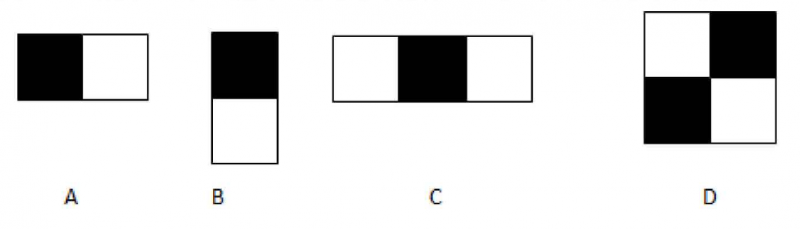
\includegraphics[width=1.0\linewidth]{figures/haarlike.png}
\caption{haar-like特征类型示意图}
\label{fig:haar-like}
\end{figure}
模板内有白色和黑色两种类型的矩形,
模板的特征值为白色矩形内的像素值的和减去黑色矩形内的像素值的和。
提取特征时使用一个滑动窗口,在原始图片中不断移位滑动,
窗口每到一个位置,就计算该窗口区域的特征值。
由于窗口可以位于图像中任意位置,并且窗口大小也可以任意改变,
因此在特征提取过程中会产生非常多的窗口,如果直接计算时间复杂度非常大,
我们可以使用积分图的方法来加速计算,
从而降低特征提取的时间复杂度。

\subsection{图像梯度}
\label{subsection:tidu}

在数学中,梯度(Gradient)是一个具有大小和方向的矢量,在
计算机视觉领域中则把梯度的模简称为梯度。
对于一副图像,我们可以将其看成二维离散函数,图像的梯度就是这个二维离散函数的导数。
和在数学中的意义相似,
图像在梯度值较大的地方,灰度值变化较大,
图像在此处可能存在边缘,在梯度值较小的地方,
灰度值变化较小,图像比较平滑。
数字图像中梯度可以用公式\eqref{eq:g}表示,
其中$dx$表示$x$方向上的梯度,可以用公式\eqref{eq:dx}得到,
$dy$表示$y$方向上的梯度,可以用公式\eqref{eq:dy}得到。
\begin{gather}
G(x,y)=dx(i,j)+dy(i,j)\label{eq:g}\\
dx(i,j)=I(i+1,j)-I(i,j)\label{eq:dx}\\
dy(i,j)=I(i,j+1)-I(i,j)\label{eq:dy}
\end{gather}

在实际求梯度时,更多的是使用差分的方法求导数的近似,
经典的图像梯度算法考虑图像中每个像素某个邻域内的灰度变化,利用边缘近似的一阶或二阶导数变化规律,对原始图像中像素邻域设置梯度算子,用梯度算子计算梯度。
常用的梯度算子有Sobel算子\cite{russ2016image}、Robinson算子\cite{russ2016image}、Laplace算子\cite{russ2016image}等。
本文使用Sobel算子计算图像梯度,
Sobel算子使用两组$3\times 3$的卷积核对图像做卷积操作,
分别求出横向和纵向的梯度近似值,
用$G_x$和$G_y$表示。
假设输入图像为$Image$,
首先将其转换成灰度图,
然后使用Sobel算子的两个卷积核对其卷积,
即可得到$G_x$、$G_y$。
卷积操作如公式\eqref{eq:gx}、\eqref{eq:gy}所示,
\begin{gather}
G_x={S\_Conv}_x*A\label{eq:gx}\\
G_y={S\_Conv}_y*A\label{eq:gy}
\end{gather}
其中,${S\_Conv}_x$表示$x$方向的卷积核,
${S\_Conv}_y$表示$y$方向的卷积核,它们的形式分别如公式\eqref{eq:sconvx}、\eqref{eq:sconvy}所示。
\begin{gather}
{S\_Conv}_x=\begin{bmatrix} -1 & 0 & +1 \\ -2 & 0 & +2\\-1 & 0 & +1\end{bmatrix}  \label{eq:sconvx}\\
{S\_Conv}_y=\begin{bmatrix} +1 & +2 & +1 \\ 0 & 0 & 0\\-1 & -2 & -1\end{bmatrix}  \label{eq:sconvy}
\end{gather}
最终图像的梯度图$G$通过公式\eqref{eq:G}得到。
\begin{equation}
G=\sqrt{G_x^2+G_y^2} \label{eq:G}
\end{equation}
为了提高计算效率,
我们使用公式\eqref{eq:jinsiG}替代\eqref{eq:G}得到$G$的近似解。
\begin{equation}
G= \left| {G}_{y} \right|+ \left| {G}_{y} \right|
\label{eq:jinsiG}
\end{equation}

这一梯度提取算法对噪声具有平滑作用,提取出的梯度特征不仅能够捕捉轮廓信息,还能弱化图像亮度的影响。

\subsection{方向梯度直方图}\label{subsection:tiquzhifangtu}

方向梯度直方图\cite{dalal2005histograms}(HOG)特征最早由法国研究员Dalal在CVPR-2005上提出,
是计算机视觉领域最常用的特征之一,
被广泛应用于物体检测中,并取得了良好的效果。
HOG特征在图像梯度的基础上,
通过统计局部区域的梯度直方图来构成更抽象的特征。

计算时我们需要用到\ref{subsection:tidu}节计算过的
横向梯度$G_x$、
纵向梯度$G_y$
和梯度$G$,
除此之外,我们还需要计算梯度的方向信息。
我们使用角度$\theta$来表示方向,
它可以使用公式\eqref{eq:tidujiaodu}计算得到。
\begin{equation}
\label{eq:tidujiaodu}
\theta (x,y)={\tan^{-1}{\frac{G_x(x,y)}{G_y(x,y)}}}
\end{equation}
接着我们将图像分成若干个单元$(cell)$,
相邻的$cell$之间不重叠,
然后我们统计每个$cell$的方向梯度直方图作为其特征。
在统计时,我们将所有的梯度方向划分为9个$bin$
作为直方图的横轴,
对应范围内梯度值的和作为直方图纵轴,
梯度方向划分方式如图\ref{fig:tiduhuafentu}所示。
\begin{figure}[htbp]
\centering
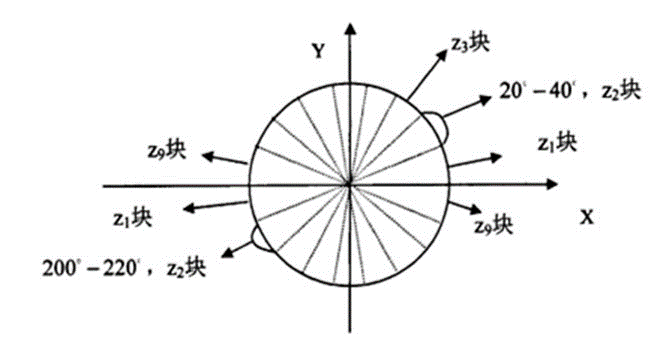
\includegraphics[width=1.0\linewidth]{figures/gradient.png}
\caption{梯度方向划分图}
\label{fig:tiduhuafentu}
\end{figure}
由于局部光照的变化和前背景的变化,
梯度值的范围可能非常大,
因此我们需要对梯度值做归一化。
归一化的方法是把各个$cell$组成空间上连通的区间$(block)$,
$block$的特征为其内部所有$cell$
的特征向量串联的结果,$block$之间可以互相重叠,我们采用滑动窗口来统计每个
$block$的特征,并将它们串联成图片的特征向量。
根据数据的大小,我们设$block$的大小
$blocksize$为
$(10,10)$,设$cell$的大小$cellsize$为
$(5,5)$,
每个$block$
包含四个$cell$。
使用滑动窗口统计$block$的特征时,
滑动窗口的步长$blockstride$设为
$(5,5)$,
这时
$block$之间有重叠,
每一个$cell$的特征都会以不同的结果多次出现在图片的特征向量中。

\subsection{局部二值模式}

局部二值模式$(LBP)$特征是一种常见的图像局部纹理特征,
该特征对光照不敏感,
并且计算方法简单,数据量小,是一种非常实用的特征。
原始的LBP算子由T. Ojala, M.Pietikäinen和 D. Harwood提出,
该算子使用像素点的$3\times 3$邻域求LBP特征。
随后Ojala等人提出了圆形LBP算子\cite{ojala2002multiresolution},将原始算子的$3\times 3$邻域扩展到任意领域,
并使其获得了灰度不变性和旋转不变性,
Ojala还提出采用“等价模式”\cite{ojala2002multiresolution}对LBP算子降维,
使得特征在减少维度的情况下仍能较好的代表图像局部纹理。

我们将LBP算子定义在
$3\times 3$的窗口内,
将窗口中心像素灰度值记为阈值$l\_thre$,接着我们将其与周围相邻的8个像素的灰度值比较,
若周围像素点的灰度值大于$l\_thre$,那么该点的位置被标记为1,
否则被标记为0,
最终中心像素点$3\times 3$
邻域内的8个点产生8个0或者1,我们将其从左上角位置开始顺时针排列成一个二进制数,将这个二进制数的大小当做中心像素点的LBP特征值,
如图\ref{fig:lbp}所示。
\begin{figure}[htbp]
\centering
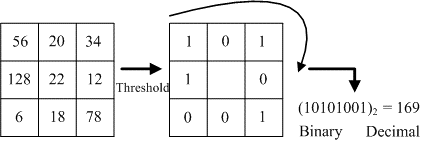
\includegraphics[width=1.0\linewidth]{figures/lbp.png}
\caption{LBP特征提取示意图}
\label{fig:lbp}
\end{figure}
从图\ref{fig:lbp}中可以看出,LBP特征的二进制数是以一定顺序编码得到的,如果图像发生旋转,其值就会发生改变,为此我们主动旋转其邻域,得到一系列LBP值,取其最小值作为最终LBP值,旋转过程如图\ref{fig:lbp2},这种方法得到的特征值拥有良好的旋转不变性。
\begin{figure}[htbp]
\centering
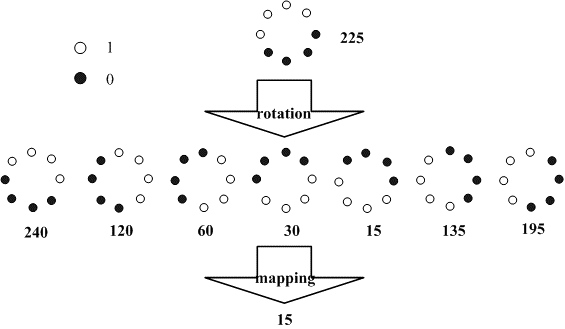
\includegraphics[width=1.0\linewidth]{figures/lbp2.png}
\caption{LBP旋转不变性示意图}
\label{fig:lbp2}
\end{figure}

接着,我们观察LBP值中从$0\rightarrow 1$或从$1\rightarrow 0$的跳变次数,
如果最多只有两次跳变,
则认为这个LBP值所对应的二进制是一个等价模式,
保留这个LBP值,否则将其划分到混合模式类,
所有混合模式类使用同一个LBP值。
最终,每个像素点都得到一个LBP值,我们并不直接使用这个值,
而是使用滑动窗口的方式获得窗口内LBP值的直方图,
将直方图作为窗口的特征,
最后将所有窗口的特征串联起来,得到整幅图像的特征。
本文实验中,滑动窗口的大小和步长和HOG特征中$block$的大小和步长相等。

\subsection{灰度共生矩阵}

灰度共生矩阵特征首先得到图像的共生矩阵,
然后通过计算该共生矩阵得到矩阵的特征值,
用这些特征值来代表图像的纹理特征。
灰度共生矩阵能够反映图像灰度方向、相邻间隔、变化幅度等综合信息。

灰度共生矩阵特征建立在图像灰度图的基础上,
因此我们首先将图片转换成灰度图$Gray$,
接着统计其灰度共生矩阵。
统计灰度共生矩阵时,我们首先取图像中任意一个点
$(x,y)$,
其灰度值记为${g}_{1}$,
取图像中另外一个点$(x+a,y+b)$,
其灰度值记为${g}_{2}$,
可以得到一个灰度值对$({g}_{1},{g}_{2})$,
当$a$、$b$固定不变,
对图像中所有的点$({x}^{'},{y}^{'})$
找对应的$({x}^{'}+a,{y}^{'}+b)$,
都可以得到一个灰度值对$({g}_{1}^{'},{g}_{2}^{'})$,
接着我们统计所有灰度值对中相同$({g}_{1}^{'},{g}_{2}^{'})$
出现的次数,
将它们排列成一个方阵,
这个方阵就是灰度共生矩阵,
方阵中在$({g}_{1},{g}_{2})$位置
上的值为$({g}_{1},{g}_{2})$出现的概率$p({g}_{1},{g}_{2})$,
$(a,b)$被称为距离差分值,
常采用不同的组合以得到不同的灰度共生矩阵,
本文使用$(1,0)$、$(0,1)$、$(1,1)$、$(-1,-1)$
作为$(a,b)$的选择,
分别对应对图片进行${0}^{\circ}$、${90}^{\circ}$、${45}^{\circ}$、${135}^{\circ}$的扫描结果。

\subsection{色彩空间}

除了传统的图像特征以外,
我们还分析了法线图色彩空间的特点。
我们将法线图记为$Normal$,
将其大小记为$M*N$,
我们用$M$表示图像宽度$width$的大小,沿着宽从左到右的方向记为水平方向,
用$N$表示图像高度$Height$的大小,沿着高从低到高的方向记为垂直方向。
首先,我们对法线图三个通道的像素值
分别在垂直和水平方向上进行投影,观察不同的投影结果。
在水平方向上的投影可以用公式
\eqref{eq:chuizhitouying}表示,
\begin{equation}
p_i=\sum_{j=0}^{N-1} I(i,j),\qquad i\in \left[ 0,M-1\right]
\label{eq:chuizhitouying}
\end{equation}
其中$p_i$表示在水平方向i点上的投影值,
$I(i,j)$表示图像中$(i,j)$位置的像素值。
接着我们对$p_i$进行归一化,
使$p_i$的值都处于$[0,1.0]$的范围内。
我们对图像在垂直方向上也做了同样的投影,
并在$B$通道水平投影上发现了明显的统计规律。如图\ref{fig:secaitongying}所示,
\begin{figure}[htbp]
\centering
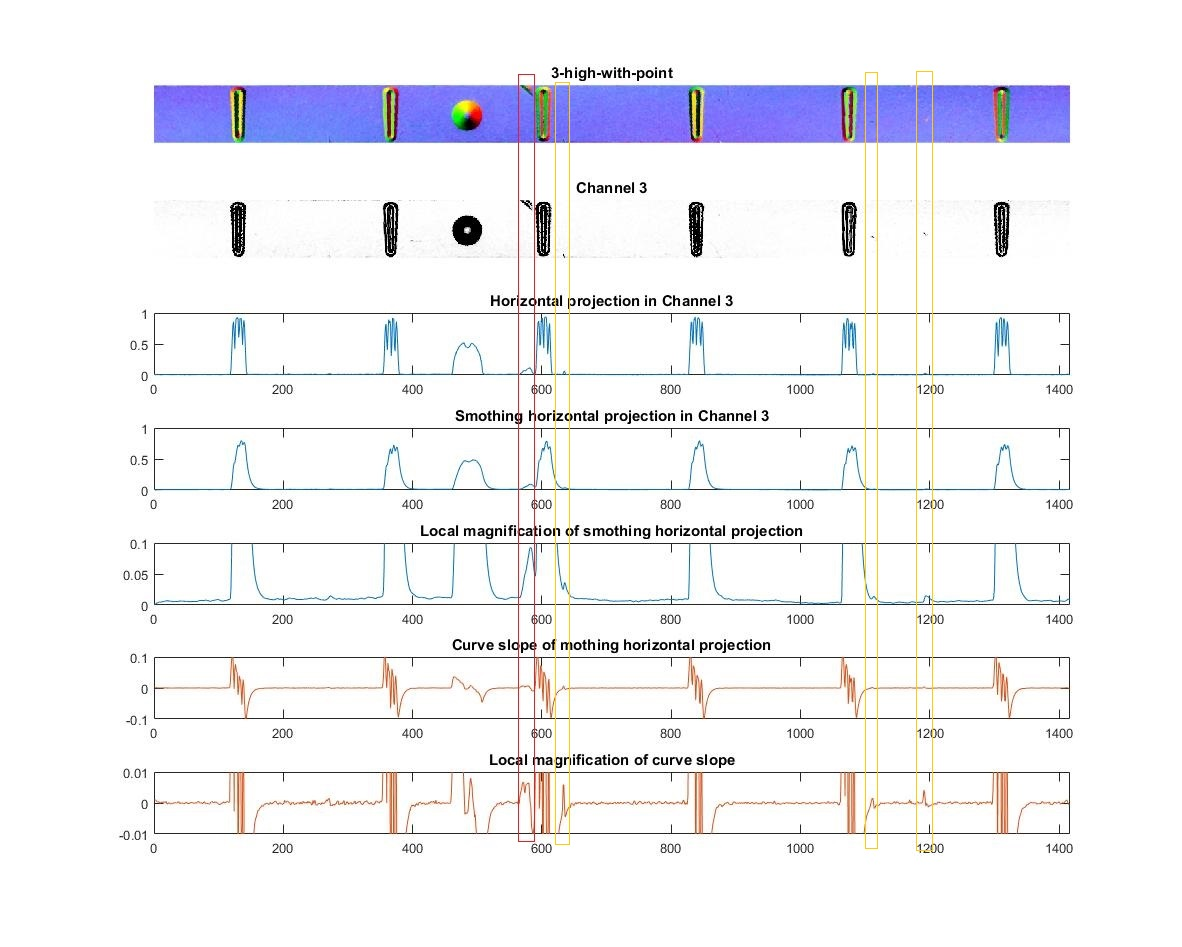
\includegraphics[width=1.0\linewidth]{figures/secaikongjian.png}
\caption{水平投影结果图}
\label{fig:secaitongying}
\end{figure}
图中$3-high-with-point$表示零件法线图,
$channel~3$表示法线图$B$通道信息,
$Horizontal~projection~in~Channel~3$表示$channel~3$水平投影的归一化结果,
$Smothing~horizontal~projection~in~Channel~3$表示对水平投影平滑后的结果,
$Local~mangnification~of~smothing~horizontal$表示平滑后的水平投影在
$[0.0,0.1]$范围内的结果,
$Curve~slope~of~smoothing~horizontal~projection$
表示平滑后水平投影的导数信息,
$Local~magnification~of~curve~slope$表示导数在$[-0.01,0.01]$范围内的结果,
红色矩形框表示零件缺陷区域,
黄色矩形框表示零件中的划痕、凹陷等区域,这些划痕、凹陷太小不足以构成缺陷。
从图中可以明显看出,在有缺陷的区域,投影值会产生剧烈抖动,
而在没有缺陷的区域,投影值非常平滑,
因此我们直接将法线图的色彩信息作为图像的一种特征。

\section{分类器设计、训练和检测}


本文使用支持向量机作为基分类器,
利用Adaboost的方法将不同的基分类器组合成一个强分类器。
在训练阶段,考虑到数据不平衡的问题,我们将数据集划分成不同的子数据集,
对于每一个子数据集训练一个强分类器,
在检测阶段,我们将不同子集训练出来的强分类器组合成一个级联检测器,
使用级联检测器进行缺陷检测。
本节首先介绍支持向量机的相关概念以及如何对其进行训练,之后介绍如何使用Adaboost将其组合成一个强分类器,最后介绍如何用级联的方法将不同的强分类器组合成级联检测器。

\subsection{支持向量机}
\label{subsection:svm}

分类一直是机器学习中非常基础和重要的领域,
常见的分类模型有随机森林\cite{breiman2001random}(Random Forest,简称 RF)、
对数几率回归\cite{周志华2016机器学习}(Logistic Regression,简称 LR)、
贝叶斯分类器以及支持向量机(SVM)等。
其中,支持向量机作为一种基于统计学习理论的监督学习算法,能在样本数量较少的情况下学习出一个不错的分类决策,
并且可以使用核函数的方法解决高维问题,
处理非线性特征的相互作用,
SVM无需依赖全部数据集,具有良好的泛化能力。
基于本文数据量小、特征维度高、线性不可分等特点,我们选择SVM作为基分类模型。

首先,
我们使用$D$来表示数据集,
并将$D$中的样本分为两类,一类是有缺陷的样本,
标记为$+1$,
一类为没有缺陷的样本,标记为$-1$,
那么$D$可以用公式\eqref{eq:shujujid}来表示,其中$x$表示样本的特征向量,$y$表示样本的标记。
\begin{equation}
\centering
D={(x_1,y_1), 
(x_2,y_2),…,(x_m,y_m)},\quad y_i\in \{-1,+1\}
\label{eq:shujujid}
\end{equation}
支持向量机通过在特征空间中构建一个超平面来划分不同的类别,
这个超平面就是这两个类的分类边界。
在特征空间中,使用公式\eqref{eq:svmgongshi}来描述这个超平面,
\begin{equation}
\centering
w^Tx+b=0
\label{eq:svmgongshi}
\end{equation}
公式中,
$x$表示特征向量,
$w=(w_1;w_2;…;w_d)$表示分类超平面的法向量,决定了超平面的方向,
$b$表示超平面的位移向量,决定了超平面到原点的距离,
根据$W$和$b$
可以唯一确定一个超平面$(w,b)$。
特征空间中点$x$到超平面$(w,b)$的距离$r$用公式\eqref{eq:r}表示,
观察该公式不难发现,$r$的大小可以通过改变$w$和$b$的值而改变。
\begin{equation}
\centering
r=\frac{\left| w^Tx+b\right|}{\lVert w\rVert}
\label{eq:r}
\end{equation}
假设超平面$(W,b)$可以将样本正确分类,
那么对于任意$(x_i,y_i)\in D$,若$y_i=+1$,则$w^T x_i+b>0$,若$y_i=-1$,则$w^T x_i+b<0$,这一条件可以用公式\eqref{eq:fenleigongshi}表示。
\begin{equation}
\centering
\begin{cases}
w^Tx_i+b>+1 ,\quad y_i=+1\\
w^Tx_i+b<-1 ,\quad y_i=-1
\end{cases}
\label{eq:fenleigongshi}
\end{equation}
并且如图\ref{fig:svm}所示,
公式\eqref{eq:fenleigongshi}中能使等号成立的点恰好是距离超平面最近的特征点,
它们被称为“支持向量”,
两个不同类支持向量到超平面的距离之和$\gamma$被称为间隔,可以用公式\eqref{eq:jiange}表示。
\begin{equation}
\centering
\gamma = \frac{2}{ \lVert w\rVert }
\label{eq:jiange}
\end{equation}
\begin{figure}[htbp]
\centering
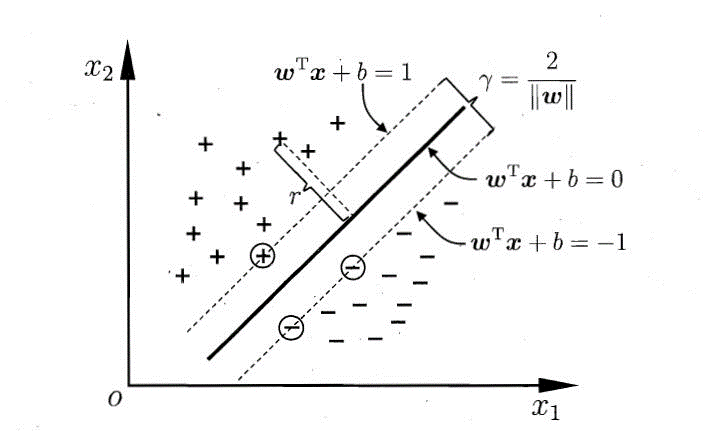
\includegraphics[width=1.0\linewidth]{figures/svm.png}
\caption{支持向量机示意图}
\label{fig:svm}
\end{figure}
SVM的核心思想是找到一个具有最大间隔的超平面,
即找到满足约束\eqref{eq:fenleigongshi}并使得$\gamma$最大的参数$w$和$b$,
可以用公式\eqref{eq:svmyueshutiaojian}表示这一约束条件。
\begin{equation}
\centering
\begin{aligned}
&\ \max_{w,b}{\frac{2}{\lVert w\rVert}}\\
&\ \mbox{s.t.}\quad y_i(w^Tx_i+b)\ge 1, \quad i=1,2,\cdots ,m.
\end{aligned}
\label{eq:svmyueshutiaojian}
\end{equation}
观察上式,为了最大化间隔,
只需要最大化${\lVert w\rVert}^{-1}$,
这等价于最小化${\lVert w\rVert}^2$,
于是我们可以将公式\eqref{eq:svmyueshutiaojian}改写为公式\eqref{eq:svmyueshutiaojian1}的形式。
\begin{equation}
\centering
\begin{aligned}
&\ \max_{w,b}{\frac{1}{2}\lVert w\rVert^2}\\
&\ \mbox{s.t.}\quad y_i(w^Tx_i+b)\ge 1,\quad i=1,2,\cdots ,m.
\end{aligned}
\label{eq:svmyueshutiaojian1}
\end{equation}
这是一个凸优化二次规划问题,
可以直接用现成的优化包求解。

虽然我们希望超平面能够将两个类完全分开,
但是现实任务中往往很难找到这样的超平面,
并且就算找到了这样的超平面,也很难判断这是不是过拟合导致的。
为了解决这一问题,我们允许某些样本不满足约束条件,只是要求不满足约束的样本尽可能少,这种方法被称为“软间隔”,它的优化目标可以用公式\eqref{eq:svmyouhuayueshu}表示,
\begin{equation}
\centering
\min_{w,b}{\frac{1}{2}\lVert w\rVert^2}+C\sum_{i=1}^{m}{y_i(w^Tx_i+b)-1}
\label{eq:svmyouhuayueshu}
\end{equation}
其中$C$是一个大于0常数,被称为正则化常数,
它需要人工优化,后面会讲到如何优化它,
$l_{0/1}$表示“$0/1$损失函数”,由于其非凸、非连续的性质,不易直接求解,实际使用时常用其他函数替代,本文使用hinge损失函数替代。

\subsection{核函数}

\ref{subsection:svm}节中描述了基本的SVM模型,
这一模型假设两个类在特征空间中线性可分,
然而在实际情况中,样本在特征空间中往往是线性不可分的。
为了解决特征空间线性不可分的问题,
SVM使用核函数的方法将数据从特征空间映射到高维空间中,
在高维空间中寻找一个可以将两个类分开的超平面。

对于原始特征空间中特征向量$x$,令$\phi(x)$表示将$x$映射到高维空间中的特征向量,
我们可以得到高维空间中对应的SVM模型,如公式
\eqref{eq:chaopingmian}所示,
\begin{equation}
\centering
f(x)=w^T\phi (x)+b 
\label{eq:chaopingmian}
\end{equation}
其中,$w$和$b$表示需要求解的模型参数,
类似于\ref{subsection:svm}中的SVM最优化形式,
这一公式的最优化形式可以用公式\eqref{eq:svmyueshutiaojian2}表示。
\begin{equation}
\centering
\begin{aligned}
&\ \min_{w,b}{\frac{1}{2}\lVert w\rVert^2}\\
&\ \mbox{s.t.} \quad y_i(w^T\phi (x_i)+b)\ge 1,\quad i=1,2,\cdots ,m.
\end{aligned}
\label{eq:svmyueshutiaojian2}
\end{equation}
求解该问题涉及到计算特征向量$x_i$和$x_j$
在高维空间中的內积${\phi (x_i)}^T \phi(x_j)$。
由于我们要将原始特征空间映射到高维空间甚至无穷维空间中,
因此直接计算${\phi (x_i)}^T \phi(x_j)$往往非常困难,
“核函数”正是为了解决这个问题,
核函数$k(.,.)$
具有如公式\eqref{eq:hehanshuxingzhi}所示的性质。
\begin{equation}
\centering
k(x_i,x_j )=\langle \phi (x_i ),\phi (x_j )\rangle=\phi (x_i )^T \phi (x_j )
\label{eq:hehanshuxingzhi}
\end{equation}
使用核函数,可以通过$x_i$和$x_j$在原始样本空间中的內积
得到其在高维空间中的內积,
使得我们可以避免直接计算高维甚至无穷维特征空间中的內积。
常用的核函数有线性核函数、多项式核函数、卡方核函数、高斯核函数、拉普拉斯核函数以及
$Sigmoid$核函数。

本文SVM算法基于libsvm\cite{CC01a}库实现,该库中预定义了很多基本核函数,可以很方便的使用。在实验中,我们测试了不同的核函数在数据集上的表现,其中高斯核表现最好也最稳定,因此,本文使用高斯核将原始特征空间映射到高维空间。
\begin{equation}
\centering
k(x_i,x_j )=\exp {⁡(-\frac{\lVert x_i-x_j \rVert ^2}{2\sigma ^2 })}
\label{eq:gaosihe}
\end{equation}

高斯核的基本形式如公式\eqref{eq:gaosihe}所示,
其中,$\sigma$表示高斯核的带宽,
是一个大于0的数,
也是使用高斯核函数时需要调整的参数。

\subsection{支持向量机训练}

在训练SVM模型时,需要人工设定的超参数有正则化常数$C$和
高斯核函数的带宽$\sigma$。
在实际训练时,
我们并不直接设定$C$和$\sigma$的值,
而是通过一定的方法来选择不同的参数,
并使用交叉验证的方法验证参数的效果,
最终使用效果最好的参数作为超参训练模型。

模型中$C$和$\sigma$是相互独立的,因此二者可以独立选择。
我们首先从$[-10,15]$中选择$\log_2⁡C$的值,
从$[-20,5]$中$\log_2⁡\sigma$的值,
然后用这组值$(C,\sigma)$作为超参训练模型,
并使用交叉验证法对模型评估,
不断重复这一过程,尝试不同的组合,
选择评估结果最好的$(C,\sigma)$作为最终的模型参数。

交叉验证法首先将原始数据集$D$划分为$K$个大小相似的互斥子集,
即$D=D_1\bigcup D_2\bigcup \dots \bigcup D_k,\quad D_i\bigcap D_j=\varnothing \quad(i\not =j)$,
本文实验中$K$取$5$,
每个子集从$D$中分层采样得到,
接着我们分别用第$k$个子集作为测试集,
用余下$k-1$个子集的并集作为训练集,
对模型进行训练和评估,
得到$k$个评估结果,
使用这$k$个评估结果的均值来评价参数的好坏。

\subsection{自适应增强算法}
\label{subsection:adaboost}

自适应增强算法(Adaboost)是boosting族算法中最具代表性的算法,
本文用它将不同的SVM模型组合成一个强分类模型。
Adaboost算法可以组合多个基学习器,
它首先训练一个基学习器,根据基学习器的表现对样本权重进行调整,
使该学习器中分类错误的样本权重更高,
然后基于调整后的样本训练下一个基学习器,
重复上述步骤直到学习器数目达到指定的值$T$,
最后将这$T$个学习器进行加权组合。

Adaboost可以用“加性模型”表示,如公式\eqref{eq:adaboostjiaxingmoxing}所示,
其中$H(x)$表示模型的最终输出,
$h_t (x)$表示基学习器的输出,
$\alpha_t$表示基学习器的权重。
Adaboost通过最小化指数损失函数优化基学习器的权重$\alpha_t$。
Adaboost在获得$H_{t-1}$之后调整样本权重,
样本权重调整的目标是使下一个基学习器$h_t$能够纠正$H_{t-1}$的错误。
\begin{equation}
H(x)=\sum_{t=1}^T{\alpha_th_t(x)}
\label{eq:adaboostjiaxingmoxing}
\end{equation}

我们使用SVM作为Adaboost的基学习器,假设第$t$个模型$h_t$的分类误差为$\varepsilon_t=1/N\left[\sum_jw_j\delta(h(x_j)\not =y_j)\right]$,
其中,$N$表示样本的数量,
$w$表示样本的权重,
那么模型权重和样本权重的更新公式
可以分别用\eqref{eq:adaboostquanzhigengxin}和\eqref{eq:adaviistshujujiquanzhigengxin}表示,
其中$D_{t}(i)$表示每个样本的权重,
$Z_t$表示使$D_t(i)$符合一个分布的归一化常数。
\begin{gather}
\alpha_t=\frac{1}{2}\ln \frac{1-\varepsilon_t}{\varepsilon_t}  \label{eq:adaboostquanzhigengxin}\\
D_{t+1}(i)=\frac{D_t(i)}{Z_t}\times
\begin{cases}
 ~~e^{-\alpha_t},\quad &\mbox{if}~~h(x_j)=y_i\\
 ~~e^{\alpha_t},\quad &\mbox{otherwise} 
\end{cases}\label{eq:adaviistshujujiquanzhigengxin}
\end{gather}

通过Adaboost训练出来的强分类器会对每个样本输出一个值$p$,
它可以被看做该样本是否为正样本的概率,
我们可以设置一个阈值$threshold$,
当$p>threshold$时,认为该样本为正样本,
也就是该样本有缺陷,
当$p\leq threshold$时,认为该样本为负样本。
显然,如果我们设置的$threshold$较高,模型会有更低的误识率,但是它的检测率也会变低,
如果我们设置的$threshold$较低,检测率会变高,但是误识率也会随之提高,这一问题可以通过增加强分类器个数,使用级联的方式做检测的方法进行优化。

\subsection{级联检测器}
\label{subsection:jilianjianceqi}

在实验过程中,
人工标记的正样本集$P$(有缺陷的样本的集合)
是小于负样本集N(没有缺陷的样本集合)的,
尤其是经过数据增强之后,样本不平衡的问题更加突出。
因此,在训练模型的时候我们并非直接使用全部训练样本训练模型,
而是将负样本分成K个子集$\{N_1,N_1,\dots,N_k\}$,这些子集的大小与$P$相同,
K是由P和N的大小确定的,取$K=ceil(|N|/|P|)$,
$|N|$表示集合$N$的元素个数,
$|P|$表示集合$P$的元素个数,
$ceil()$表示向上取整函数。
子集的划分使用随机抽样的方法,
我们首先从$N$中随机无放回的抽取$|P|$个元素组成第一个子集$N_1$,
接着不断重复这一过程直到得到$k-1$个子集,
这时$N$中剩余的元素个数为$N_{rmain}$,
我们从得到的$k-1$个子集中随机的抽取$|P|-N_{rmain}$个元素,
将这些元素和$N$中剩余的元素组成第K个子集。
我们分别将这$K$个子集和正样本集$P$组成一组子数据集,
从而得到$k$个正负样本均衡的子数据集。
对于每个子数据集,我们训练一个强分类器,
最后使用级联\cite{viola2001rapid}(Cascade)的方式将这些分类器用于缺陷检测。

\begin{figure}[htbp]
\centering
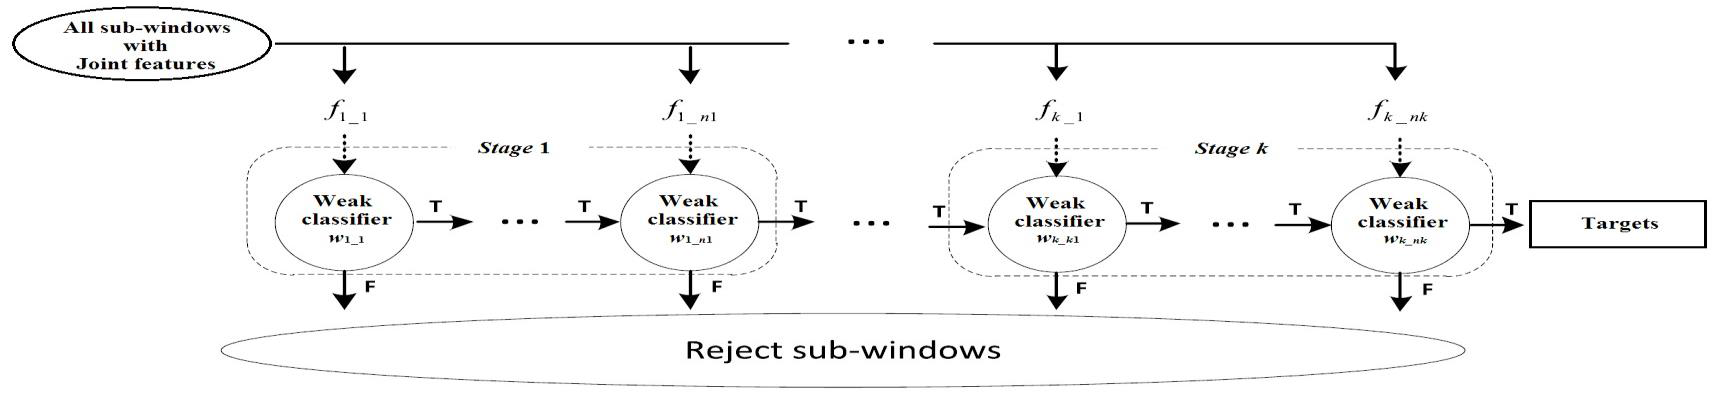
\includegraphics[width=1.0\linewidth]{figures/cascade.png}
\caption{级联分类器模 型图}
\label{fig:cascade}
\end{figure}
级联分类器流程如图\ref{fig:cascade}所示,首先使用Adaboost组合SVM训练出$K$个不同的强分类器,
我们将每个强分类器的检测视作一个$stage$,每个$stage$中基分类器的个数为$n$。
在检测的时候使用滑动窗口的方式将输入图片划分成不同的窗口,首先将所有的窗口用第一个强分类器进行分类,即用$stage~1$分类,
将所有检测为正常的窗口归到$Reject~sub-windows$中,
认为这些窗口为正常零件,
将所有检测为缺陷的窗口送往下一个$stage$中,
重复这一步骤,
直到所有的强分类器都检测这一窗口为缺陷,将其视为缺陷,归入$targets$中。

由于在缺陷检测中,一旦发生漏检,缺陷零件流出,往往会造成重大损失,
相对于漏检,误检一个、几个甚至几十个零件所带来的损失往往可以忽略不计,我们需要尽可能的提高检测率,在检测率尽可能高的情况下降低误识率。
我们在选择强分类器阈值时,选择能使模型达到最大检测率的最大值。


\section{实验结果和分析}
\label{section:shiyanjieguo}

本节首先描述实验环境,然后描述实验过程和实验结果。实验结果主要包括两个部分,
第一个部分为特征提取结果,
第二个部分为缺陷检测结果。

\subsection{实验环境}

实验环境为一台拥有$\mbox{Intel Core}
~I7-7700$处理器的计算机,
该机器的系统为$Win7$,
处理器内存为$8GB$。
本文使用的语言主要有matlab\cite{MATLAB:2017}、C++、python等。
用到的库主要有matlab\cite{MATLAB:2017}、OpenCV\cite{opencv_library}、libsvm\cite{CC01a}等。

\subsection{特征提取结果}

我们使用\ref{section:tezhengtiqu}节中介绍的特征提取方法对数据进行特征提取。
在特征提取过程中,
我们并不是在分割后的图片上提取,
而是先提取整幅图片的特征,
再使用滑动窗口的方法得到分割图片的特征,这种算法大大加速了整个计算流程。

以梯度特征为例,我们首先计算整幅图像的梯度,
用矩阵的形式保存梯度信息,
图片大小用$N\times M$表示,图像中的像素点位置用$(x,y)$表示,
保存梯度信息的矩阵大小为$N\times M$,
矩阵中$(x,y)$位置的值代表了对应图片$(x,y)$位置的梯度信息,
在使用滑动窗口对主表面图进行分割时,只需要选取对应窗口的梯度信息,
即可得到分割后图片的梯度特征。

我们选择一组数据为例介绍特征提取结果。如图\ref{fig:butogndengguangzhankaitu}所示为该组数据在不同光照条件下拍摄的照片和法线图,
其中$Top$为顶部光源照射时的拍摄照片,可以看到由于金属零件表面高光的原因,照片中只有特别明显的缺陷和划痕才能看到,细节部分被完全掩盖了;
$East$、$West$、$South$、$North$分别代表了东部灯光组、西部灯光组、南部灯光组和北部灯光组亮照射时的照片,
这些照片色彩丰富,纹理清晰,
拥有丰富的细节,即是非常微小的纹理、裂缝、划痕、污点也不会丢失,
这些丰富的细节虽然提供了大量信息,但其中干扰信息过多,无疑增大了缺陷检测的难度;
$Normal$表示法线主表面图,
该图能够很好地滤除无用纹理和色彩信息,同时保留由裂缝、划痕等缺陷造成的表面信息。

\begin{figure}[htbp]
\centering
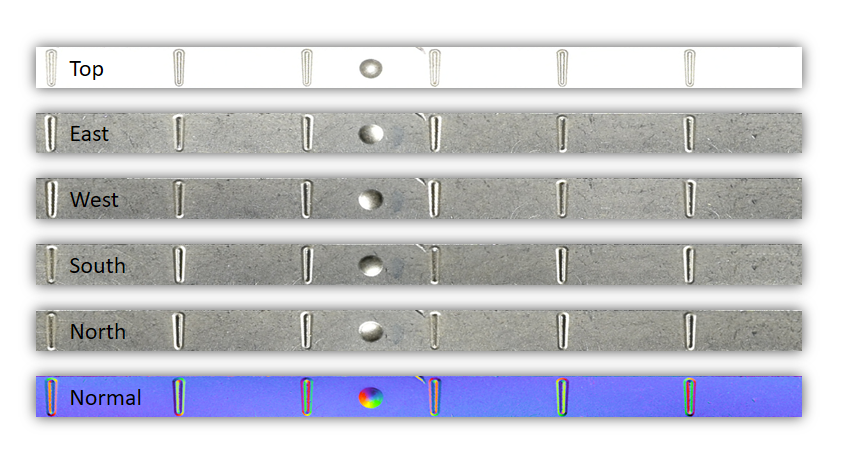
\includegraphics[width=1.0\linewidth]{figures/butongdengguangzhankaitu.png}
\caption{不同光照下主表面结果图}
\label{fig:butogndengguangzhankaitu}
\end{figure}

为了进一步对比不同数据对分类的影响,
我们使用canny\cite{canny1983finding}算子提取它们的边缘信息。
canny算子在提取边缘信息的时候,
需要设定两个滞后性阈值$threshold1$和$threshold2$,
其中二者的较小值的被用于边缘连接,较大值被用来控制强边缘的初始段,
我们将两个阈值分别设为$100$和$300$,同时设定canny算子中sobel算子的卷积核大小为$3$。
\begin{figure}[htbp]
\centering
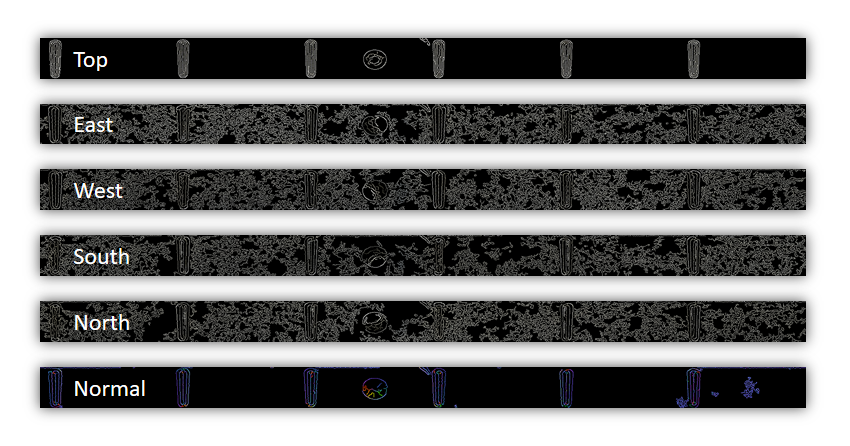
\includegraphics[width=1.0\linewidth]{figures/butongdengguangcanny.png}
\caption{不同光照下边缘检测结果图}
\label{fig:butongdengguangcanny}
\end{figure}
得到的结果如图\ref{fig:butongdengguangcanny}所示,
该组图的命名规则和图\ref{fig:butogndengguangzhankaitu}一样。
从边缘提取图片中的边缘密度可以看出,
$Top$和$Normal$边缘相对简单,和真正的边缘比较接近,
但是$Top$中边缘信息太少,有些缺陷的边缘甚至没有被提取出来,
而$Normal$中没有这个问题;
不同方向光源下的照片边缘过多,这些边缘大多由图片的色彩、纹理等造成,和缺陷检测无关。


\begin{figure}[htbp]
\centering
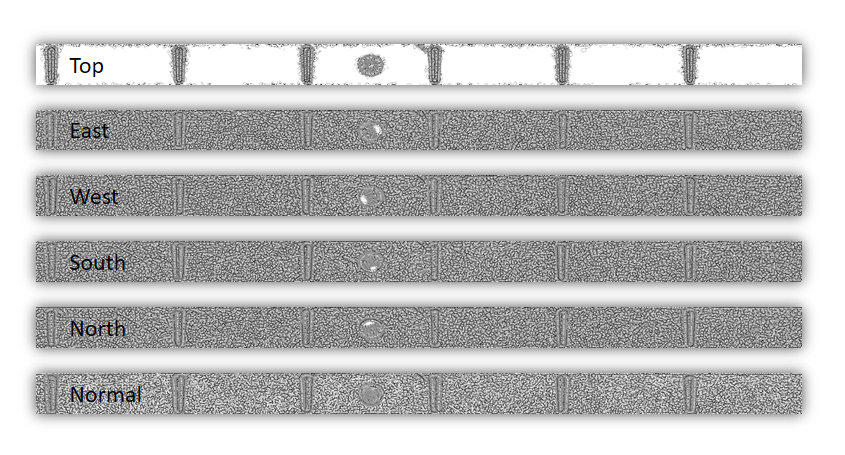
\includegraphics[width=1.0\linewidth]{figures/butongdengguanglbp.png}
\caption{不同光照下LBP特征提取结果图}
\label{fig:butongdengguanglbp}
\end{figure}
\begin{figure}[htbp]
\centering
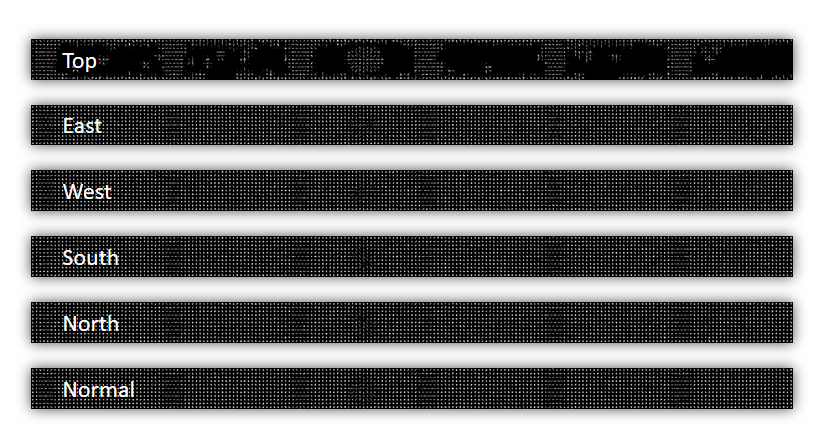
\includegraphics[width=1.0\linewidth]{figures/butongengguanghog.png}
\caption{不同光照下HOG特征提取结果图}
\label{fig:butongengguanghog}
\end{figure}

上述特点还体现在其它特征提取结果中。
如图\ref{fig:butongdengguanglbp}
和图\ref{fig:butongengguanghog}分别展示了提取LBP特征和HOG特征的结果,
由于$Top$过滤掉了太多信息,无论是LBP特征还是HOG特征都会出现大量空白,甚至在有缺陷的地方也出现空白;而不同方向光源下照片的特征提取结果则过于密集,没有明显规律;
法线图的特征提取结果则综合了二者的优点,具有良好的性质。

\subsection{缺陷检测结果}
\label{subsection:chuantongjiancejieguo}

本文使用召回率($recall$,记为$REC$)、
查准率($precision$,记为$PRE$)、
漏检率( $missing~detection~rate$,记为$MDR$)、
误检率($false~detection~rate$,记为$FDR$)
作为模型评价标准,
其中漏检率是最重要的标准,误检率往往不是特别重要。
假设总共用来测试的零件数量为$N$,
其中正样本即有缺陷的样本数量为$N_p$,
负样本即没有缺陷的样本个数为$N_n$,
显然有$N=N_p+N_n$。其中,$N_p$个正样本中分类正确的个数为$TP$,
分类错误的个数为$FN$,
$N_n$个负样本中分类正确的个数为$TN$,
分类错误的个数为$FP$。
我们可以使用公式\eqref{eq:rec}、\eqref{eq:pre}、\eqref{eq:mdr}、\eqref{eq:fdr}
计算评估指标。
\begin{gather}
REC=\frac{TP}{TP+FN}\label{eq:rec}\\
PRE=\frac{TP}{TP+FP}\label{eq:pre}\\
MDR=\frac{FN}{TP+FN}\label{eq:mdr}\\
FDR=\frac{FP}{FP+TN}\label{eq:fdr}
\end{gather}

经过数据预处理之后,我们得到1128张有缺陷的正样本图片和6328张无缺陷的负样本图片,
接着我们将其划分为7个子数据集,每个数据集中各包含1128个正样本和1128个负样本。
我们首先选择一个子数据集,
在这个子数据集上,
分别使用不同灯光条件下的照片和法线图的
HOG特征作为输入,训练一个强分类器,
并设置阈值为0.9来分类。
典型分类结果如图\ref{fig:chuantongjiancejieguo}所示,
其中黄色矩形标出了检测为缺陷的窗口,
$(c)$、$(d)$、$(e)$、$(f)$
分别表示东、西、南、北四组光照图片的检测结果。因为南、北和东、西两组结果非常相似,
因此我们分别展示两组数据的结果,一组零件包含两个缺陷,结果为图中$(c)$和$(e)$,
一组零件没有缺陷,结果为图中$(d)$和$(f)$。
在有缺陷的零件检测结果中,并没有检测出所有缺陷,并且出现大量误检,没有缺陷的零件同样出现大量误检;
$(b)$表示$(c)$、$(e)$相同零件使用顶部光源拍照图片得到的检测结果,
结果中误检大大减少,
但它也没有检测出所有缺陷,我们推测这是由于输入数据过滤掉了太多信息导致;
$(a)$表示法线图特征的检测结果,
对于这个零件,它检测出了所有的缺陷信息,并且没有任何误检。
\begin{figure}[htbp]
\centering
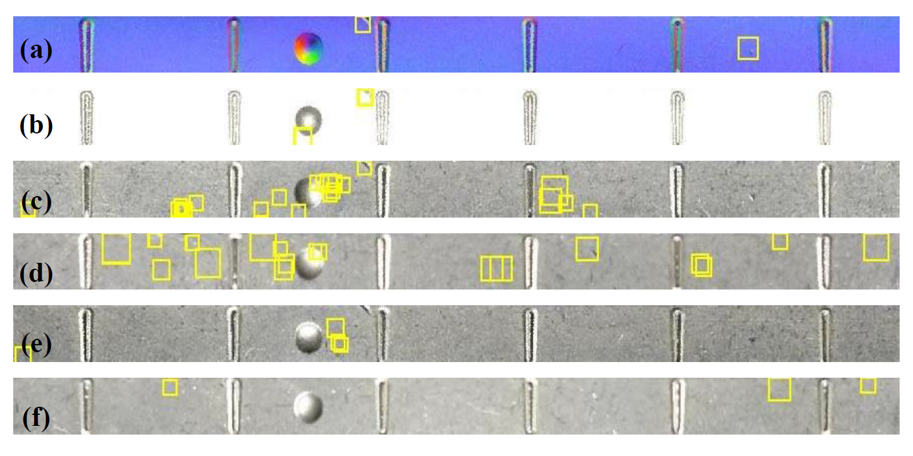
\includegraphics[width=1.0\linewidth]{figures/chuantongjiancejieguo.png}
\caption{不同输入检测结果示意图}
\label{fig:chuantongjiancejieguo}
\end{figure}
对于本文采用的评价指标结果如表\ref{tab:butongguanzhaojiancejieguo}所示,从表中不难看出,
使用不同方向光源下的照片作为数据,得到的结果非常差,
任何一项评价指标都毫无亮点,
使用顶部灯光组照片得到的结果在$recall$,$precision$上略有起色,但仍难以达到理想效果,
而使用我们提取的法线图作为数据,可以得到比较好的结果。

\begin{table}
\centering
\begin{tabular}{cccccp{38mm}}
\toprule
\textbf{输入类型} & \textbf{REC} & \textbf{PRE} & \textbf{MDR} & \textbf{FDR}\\
\midrule
\mbox{东部灯光组} & 0.6071 & 0.2484 & 0.3929 & 0.3279\\
\mbox{西部灯光组} & 0.6249 & 0.2664 & 0.3751 & 0.3072\\
\mbox{南部灯光组} & 0.7143 & 0.3091 & 0.2857 & 0.2850\\
\mbox{北部灯光组} & 0.7428 & 0.3134 & 0.2572 & 0.2905\\
\mbox{顶部灯光组} & 0.8574 & 0.5022 & 0.1426 & 0.1517\\
\mbox{法线图} & 0.9293 & 0.5981 & 0.0707 & 0.1115\\
\bottomrule
\end{tabular}
\caption{不同光照条件下检测结果表}
\label{tab:butongguanzhaojiancejieguo}
\end{table}

接着,我们分别使用法线图的梯度特征、HOG特征、LBP特征、GLCM特征、Haar-like特征、以及本身的颜色信息作为模型的输入特征,
在7个子数据集上训练出不同的强分类器,
并使用级联的方法做检测,
实验结果如表\ref{tab:butongtezhengjieguobiao}所示,
从中不难看出,使用梯度特征、HOG特征和颜色信息$(RGB)$
得到的结果要明显好于使用LBP特征、GLCM特征和Haar-like特征得到的结果。
我们认为梯度特征、HOG特征本身能更好的反应图像中像素值的变化情况,
而在法线图中,像素值的变化反应了零件表面的高低起伏变化情况,和缺陷本身关系密切,
并且,法线图的颜色信息同样反应了零件表面的变化情况。
有趣的是,测试的时候我们发现,有时HOG特征训练出来的模型反而不如直接使用梯度信息训练的模型效果好。
我们认为,法线图本身已经可以当做一个优秀的特征了,在此基础上提取HOG特征反而可能会丢失某些信息。
在此基础上,我们使用法向图的梯度信息、HOG特征和颜色信息作为组合特征,
重新训练出一个分类模型,取得了较好的结果,其结果在表\ref{tab:butongtezhengjieguobiao}展示。

\begin{table}
\centering
\begin{tabular}{cccccp{38mm}}
\toprule
\textbf{输入类型} & \textbf{REC} & \textbf{PRE} & \textbf{MDR} & \textbf{FDR}\\
\midrule
\mbox{Haar-like} & 0.8214 & 0.4677 & 0.1786 & 0.1669\\
\mbox{LBP} & 0.8932 & 0.5374 & 0.1062 & 0.1372\\
\mbox{Gredient} & 0.9114 & 0.5727 & 0.0886 & 0.1214\\
\mbox{HOG} & 0.9642 & 0.7207 & 0.0358 & 0.0667\\
\mbox{GLCM} & 0.7862 & 0.4921 & 0.2183 & 0.1448\\
\mbox{HOG+Gredient+RGB} & 0.9915 & 0.8158 & 0.0085 & 0.0400\\
\bottomrule
\end{tabular}
\caption{不同特征检测结果表}
\label{tab:butongtezhengjieguobiao}
\end{table}

最后,我们还测试了不同分类器的检测速度,从表\ref{tab:tezhengcesudu}可以看出,
检测速度最快的特征是haar-like特征,
LBP特征比haar-like特征略慢,
其次是梯度特征,
HOG特征需要在梯度特征的基础上进一步加工,速度比梯度特征慢,但并没有慢多少,
GLCM特征速度最慢,这是由于其特征提取时间复杂度最高,
本文综合梯度信息、HOG特征和颜色信息做检测速度比HOG特征稍慢,但仍然非常快。
\begin{table}
\centering
\begin{tabular}{cccccccp{38mm}}
\toprule
\mbox{特征种类} & \mbox{Haar-like} & \mbox{LBP} & \mbox{Gredient} & \mbox{HOG} & \mbox{GLCM} & \mbox{HOG+Gredient+RGB}  \\
\mbox{检测速度} & 11ms & 17ms & 16ms & 22ms & 486ms & 25ms \\
\bottomrule
\end{tabular}
\caption{不同特征检测速度表}
\label{tab:tezhengcesudu}
\end{table}



%深度学习方法
\chapter{基于深度学习的缺陷检测}


本章将详细介绍如何将法线图应用到深度学习中,对零件进行缺陷检测。
首先我们会介绍一些深度学习的基本概念,
包括卷积层、激活函数、池化层、全连接层等,
接着介绍本文使用的神经网络模型的网络结构,
最后介绍如何对模型进行训练和测试,并给出实验结果和分析。

\section{基本概念}

本文使用卷积神经网络($Convolutional Neural Networks,\mbox{简称}~CNN$)结构进行缺陷检测。
卷积神经网络是一种层次模型,
它的输入是一张图像,
接着通过卷积($convolution$)操作、
池化\cite{chechik1998synaptic}($pooling$)操作和非线性激活函数($non-linear~activation~function$)映射等一系列操作的堆叠,
逐渐从原始图像提取出高维特征,
最后通过全连接层和输出层连接,
将目标任务(分类、回归等)形式化为目标函数,
并使用损失函数($loss function$)
计算预测值和真实值之间的损失($loss$),
使用反向传播算法\cite{周志华2016机器学习}($back-propagation algorithm$)将损失从后向前传播,更新参数,
如此反复直到模型收敛。

好的卷积神经网络模型得益于良好的网络结构设计,
而一个复杂精妙的网络结构往往由诸多基本结构组成,
本节首先介绍构成神经网络的一些基本结构,
这些结构将在接下来的网络结构以及实验等部分用到,
接着介绍网络模型的损失函数和优化方法。

\subsection{卷积层}

卷积是卷积神经网络中的基础操作。所谓卷积,就是使用一个固定大小的卷积核,通过滑动窗口的形式和图像对应区域做內积(逐个元素相乘再求和)操作,此时卷积核为一个固定大小的矩阵,这些矩阵的值即为该卷积核的权值。一般我们使用正方形的卷积核,并且其大小取奇数,常用的有$1\times 1$、$3\times 3$、$5\times 5$的卷积核,卷积核的大小即对应了滑动窗口的大小。
每完成一次卷积操作,卷积核移动一个位置,移动的大小记为卷积步长($stride$)。
因为图像是二维的,为了卷积整幅图像,需要卷积核向两个方向移动,因此卷积步长也是二维的,一般取$1\times 1$。

不难看出,卷积是一种局部操作,通过一定大小的卷积核作用于图像的局部区域,从而得到图像的局部信息,通过层层卷积,高层的卷积核可以扫过的信息会覆盖原始图片的更大区域,提取图像更高层的信息。需要注意的是,图片的底层特征往往与其在图片中的位置无关,因此我们在对图像做一次卷积时使用权值相同的卷积核,这被称为“权值共享”。权值共享大大减少了卷积层的参数,起到了防止过拟合的作用。

\subsection{激活函数}

激活函数层又称为非线性映射层,其引入正是为了增加整个网络的表达能力(非线性)。如果没有激活函数层,那么整个网络仍可以看作是若干线性操作的堆叠,只能起到线性映射的作用。直观的看,激活函数模拟了神经元的特点:接收一组输入信号并产生输出。
激活函数的输入往往是卷积层卷积之后得到的值,因此通常激活函数层紧跟着卷积层,被合并为一层。

从定义来看,几乎所有的连续可导函数都可以作为激活函数,但是目前常见的多是分段性和具有指数形状的非线性函数,
本小节将介绍几种最基础的激活函数,
包括$Sigmoid$\cite{魏秀参解析卷积神经网络}函数、$Tanh$\cite{魏秀参解析卷积神经网络}函数和$ReLU$\cite{魏秀参解析卷积神经网络}函数。

\subsubsection{$Sigmoid$ 函数}

$Sigmoid$是使用范围最广的一类激活函数,
它是具有指数函数形状的激活函数。该函数的定义如公式\eqref{eq:sigmoid}所示。
\begin{equation}
\centering
f(x)=\frac{1}{1+e^{-x}}
\label{eq:sigmoid}
\end{equation}
其函数形状如图\ref{fig:Sigmoid}所示,从图中可以明显看出,经过$Sigmoid$型函数作用后,输出响应值的值域被压缩到$(0,1)$之间。
$Sigmoid$ 有其有利的一面,它在物理意义上最为接近生物神经元,并且$(0,1)$的输出范围可以理解为一个概率分布。
但是不难看出,
对于大于5(或小于-5)的值,无论多大(或多小)都会被压缩为1(或0),此部分的梯度会接近0,
从而导致在误差反向传播过程中该区域的误差很难传播,进而导致模型无法收敛,这一现象被称为“梯度消失”。
梯度消失可以被其它优化方法缓解,如Batch Normalization\cite{ioffe2015batch}。
\begin{figure}[htbp]
\centering
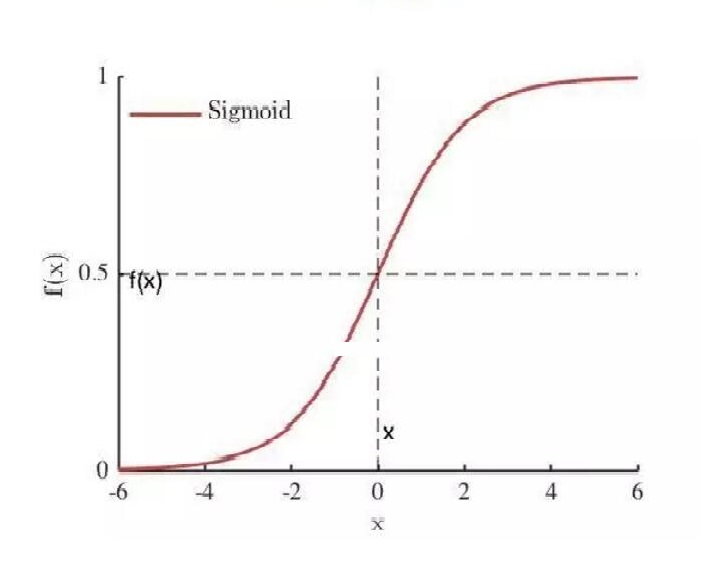
\includegraphics[width=0.6\linewidth]{figures/sigmoid.png} 
\caption{$Sigmoid$激活函数示意图}
\label{fig:Sigmoid}
\end{figure} 

\subsubsection{$Tanh$ 函数}

$Tanh$激活函数又被称为双正切函数,
其形状与$Sigmoid$函数类似,都能将输出压缩到$(0,1)$,
但是该函数输出的均值比$sigmoid$函数更接近0,在训练时收敛速度更快。
$Tanh$函数形式如公式\eqref{eq:tanh}所示。
\begin{equation}
tanh⁡(x)=\frac{1-e^{-2x}}{1+e^{-2x}}
\label{eq:tanh}
\end{equation}
$Tanh$函数形状如图\ref{fig:tanh}所示,不难看出,
$tanh$函数在$x$比较大或者比较小的时候仍会出现梯度消失的现象。
\begin{figure}[htbp]
\centering
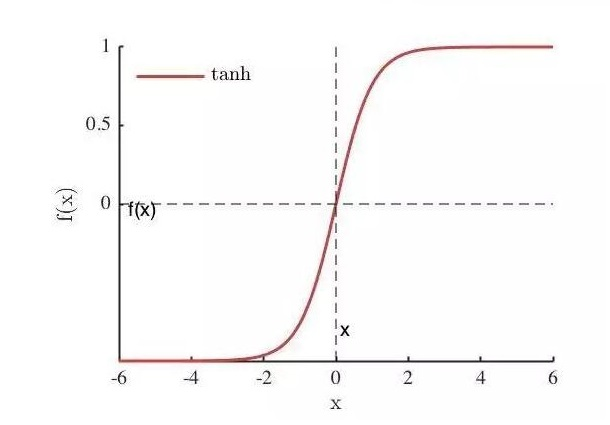
\includegraphics[width=0.6\linewidth]{figures/tanh.png}
\caption{$tanh$激活函数示意图}
\label{fig:tanh}
\end{figure}

\subsubsection{$ReLU$ 函数}

$ReLU$\cite{nair2010rectified}是由Nair和Hinton在2010年提出的,
现已成为深度学习中最常用的激活函数之一。$ReLU$函数实际上是一个分段函数,其函数形式如公式\eqref{eq:relu}所示。
\begin{equation}
\centering
ReLU(x)=\max\{0,x\}
\label{eq:relu}
\end{equation}
与前两个激活函数相比,$ReLU$函数的梯度在$x\geq 0$时为1,反之为0,如图\ref{fig:relu}所示,
在$x\geq 0$的部分,该函数完全消除了梯度消失的情况,并且$ReLU$的计算复杂度更低,
在实际应用中能够更快的收敛。
$ReLU$的主要缺陷是在$x<0$时,
梯度为0,函数对这部分的卷积结果无法响应,
因此输入一旦变为负值将再无法影响网络的训练。
这一缺陷可以通过$Parametric~Rectified~Linear~Unit(PReLU)$\cite{he2015delving}来改善。
\begin{figure}[htbp]
\centering
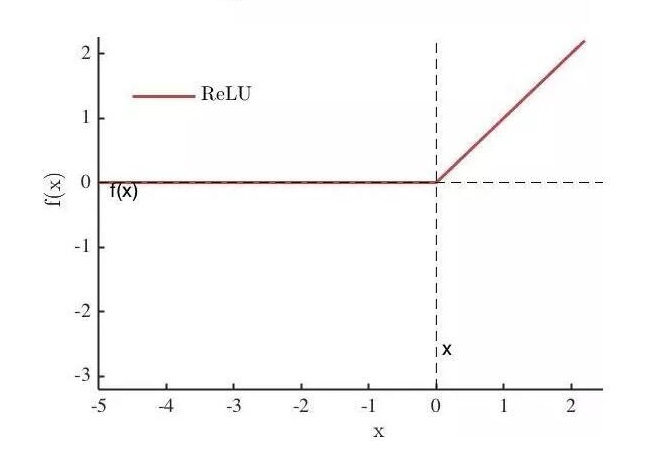
\includegraphics[width=0.6\linewidth]{figures/relu.png}
\caption{$ReLU$激活函数示意图}
\label{fig:relu}
\end{figure}

\subsection{池化层}

池化层一般采用平均池化($average-pooling$)或最大池化($max-pooling$)。
类似于卷积操作,池化层选择一个滑动窗口,取窗口中像素值最大值(最大池化层)或者平均值(平均池化层)作为池化操作的输出,可以对特征进行降维。从操作的角度来讲,池化层可以看做是一个用$p-$范数($p-norm$)作为非线性映射的“卷积”操作,当$p$趋近于正无穷时就是最大池化层。
与卷积层不同的是,池化层不需要设定参数,
使用时只需要指定池化层类型、池化操作的步长和核的大小即可。
从图像处理的角度来看,池化层可以被视为一种“降采样”,
一般卷积操作之后得到的特征可能会包含较多冗余信息,池化层的引入可以对特征进行降维和抽象,在一定程度上预防过拟合。
虽然池化层不是卷积神经网络中必须的,但是由于其良好的性质,往往会在卷积层之后使用池化层对特征降维。

\subsection{全连接层}

全连接层往往在整个卷积神经网络的最后一层或几层,起到“分类器”的作用。在这一层,每一个神经节点都会与上一层中的所有节点相连,因此全连接层往往含有较多参数。
如果说卷积层、激活函数和池化层是用来将原始数据映射到高维特征空间中的话,
那么全连接层就起到将特征映射到样本的标记空间中的作用。
实际应用中全连接层可以通过卷积操作实现,
当其前一层为全连接层时,可以通过$1\times 1$的卷积核实现,
当其前一层为卷积层时,可以通过与前一层特征维度大小一致的卷积核做全局卷积实现。

\subsection{损失函数}
\label{subseciont:sunshihanshu}

损失函数又被称为目标函数,被用来衡量预测值和真实样本标记之间的误差。在卷积神经网络中,
分类问题常用交叉熵损失函数作为目标函数,回归问题常用$l_2$损失函数作为目标函数。
\begin{equation}
\centering
L_{loss}=-\frac{1}{N}\sum_{i=1}^N(y_i\log{\hat{y_i}+(1-y_i)\log{(1-\hat{y_i})}})
\label{eq:lloss}
\end{equation}
本文将缺陷检测定义为一个二分类问题,
使用交叉熵损失函数$L_{loss}$作为目标函数,
其公式定义如\eqref{eq:lloss}所示,
其中N表示样本的数量,
$L_{loss}$表示整体损失。
$y_i$表示样本标签,当样本为缺陷样本时,
$y_i$值为1,
当样本为正常样本时,$y_i$值为0,
$\hat{y_i}$表示模型的输出,
它可以被看作该样本是缺陷样本的概率。
最终模型会输出样本为每个类的概率,
我们取概率最大的类作为最终预测的类。

\subsection{优化方法}

有了目标函数之后就可以针对目标函数优化网络参数,深度卷积神经网络通常采用随机梯度下降类的优化算法对模型参数优化。本节将介绍几种最常用的优化算法。

\subsubsection{随机梯度下降}

随机梯度下降算法($Stochastic~Gradient~Descent,\mbox{简称}~\mbox{SGD}$)是神经网络中最基础的优化算法,它根据误差的一阶梯度信息对参数调整,参数的更新策略可以用公式\eqref{eq:sgd}表示,
\begin{equation}
\centering
w=w-\eta \cdot dw
\label{eq:sgd}
\end{equation}
其中,$dw$表示误差对参数w的导数即梯度,它依赖于当前数据在目标函数上的误差,
我们利用误差的反向传播算法对其求解;
$\eta$表示学习速率,
是SGD算法中唯一的超参数,表示当前梯度值对网络参数更新的影响程度。
SGD算法收敛效果稳定,但是收敛速度较慢,并且,权值容易被困在鞍点,即$dw=0$的点,导致模型无法完全优化。SGD中学习率的设定也是一个问题,在选择学习率的时候,过大的学习率可能导致模型在训练阶段后期来回震荡,无法收敛,过小的学习率又会影响收敛速度。

\subsubsection{基于动量的随机梯度下降法}

受物理学研究的启发,
发展出了基于动量\cite{qian1999momentum}($momentum$)的随机梯度下降算法,
该算法通过前几轮训练积累的“动量”信息辅助参数更新,更新策略用公式\eqref{eq:momentum}表示,
\begin{equation}
\begin{aligned}
\centering
v & =\mu \cdot v-\eta \cdot dw \\
w & =w+v
\end{aligned}
\label{eq:momentum}
\end{equation}
公式中,$\mu$为动量因子,表示动量对整体梯度更新的影响程度,
一般$\mu$取0.9;
$v$表示动量,在梯度方向相同的方向逐渐增大,
在梯度方向不同的方向逐渐变小;
$\eta$为学习率,
表示梯度$dw$对动量的影响。
基于动量的随机梯度下降法可以抑制SDG中会出现的震荡现象,
还可以帮助跳出鞍点,找到参数的更优解。

\subsubsection{RMSProp算法}

RMSProp($root~mean~square~prop$)算法\cite{hinton2012neural}可以针对学习率做动态的调整。这一算法的更新策略如\eqref{eq:rmsprop}所示,
\begin{equation}
\begin{aligned}
\centering
Sdw & =\beta \cdot Sdw-(1-\beta )dw^2 \\
w & =w- \alpha \frac{dw}{\sqrt{Sdw}+\varepsilon }
\end{aligned}
\label{eq:rmsprop}
\end{equation}
公式中加入了w的二阶导数对$Sdw$进行更新,在更新$w$的时候使用用$w$的梯度除以$Sdw$的平方根作为学习对象,
这使得对于不同的w可以有不同的学习率。其中$\varepsilon$只是为了防止分母变为0,本身对算法的意义不大,一般置为${10}^{-6}$,$\beta$为衰减因子,用于消除算法对全局学习率$\alpha$的依赖,
较大的$\beta$会促进网络更新,较小的$\beta$会抑制网络更新,一般可以取0.9,$\alpha$可以取1。

\subsubsection{Adam算法}

Adam\cite{kingma2014adam}算法用梯度的一阶矩估计和二阶矩估计动态调整每个参数的学习率,并且经过偏置校正后,每一次迭代学习率都有一个确定的范围,可以使得参数更新更加平稳。算法使用公式\eqref{eq:adam}调整参数$w$,调整时首先初始化$Vdw=0$,$Sdw=0$,
接着不断迭代更新参数,直到模型收敛。
\begin{equation}
\begin{aligned}
\centering
&Vdw  =\beta_1 \cdot Vdw-(1-\beta_1 )dw \\
&Sdw  =\beta_2 \cdot Sdw-(1-\beta_2 )dw^2 \\
&Vdw^{corrected}  =\frac{Vdw}{1-\beta_1^t}\\
&Sdw^{corrected}  =\frac{Sdw}{1-\beta_2^t}\\
&w  =w- \alpha \frac{Vdw^{corrected}}{\sqrt{Sdw^{corrected}}+\varepsilon }
\end{aligned}
\label{eq:adam}
\end{equation}
可以看出,Adam算法也需要指定参数,其中$\varepsilon$是为了防止分母为0,
使用${10}^{-6}$即可;$\beta_1$为第一矩参数,可以使用0.9;$\beta_2$为第二矩参数,
可以使用0.999。
该算法既考虑了动量又可以针对不同的参数调整学习率,常常具有较快的收敛速度和较好的效果。本文使用Adam算法对模型进行优化。

\section{深度学习模型}

本文使用VGG-11\cite{simonyan2014very}模型,
并对其进行了一定修改。
模型结构如图\ref{fig:VGG}所示,
图中用不同颜色的矩形标示出了不同种类的网络层。
第一层为输入层,输入图片的大小为$224\times224\times3$;
黑色矩形表示卷积层,
卷积核大小为$3\times3$,
步长为2。
论文中VGG11的卷积层后面紧跟$ReLU$激活层,
本文在卷积层之后、$ReLU$层之前加入了批归一化($Batch~Normalization$)层,
批归一化层由Sergey loffe和Christian Szegedy等人提出,
可以将数据归一化至均值为0、方差为1的分布。
这种方法有两个好处:首先它把输入的均值、方差规范化,保证了每一层的输入分布不发生改变,能够加快模型收敛;
其次它能起到轻微正则化的作用,预防过拟合。
红色矩形表示最大池化层,池化窗口大小为$2\times2$,步长为2。
浅蓝色矩形表示全连接层和紧随其后的$ReLU$激活层。
深蓝色矩形表示全连接层。
褐色矩形表示$Softmax$层,用于分类。

\begin{figure}[htbp]
\centering
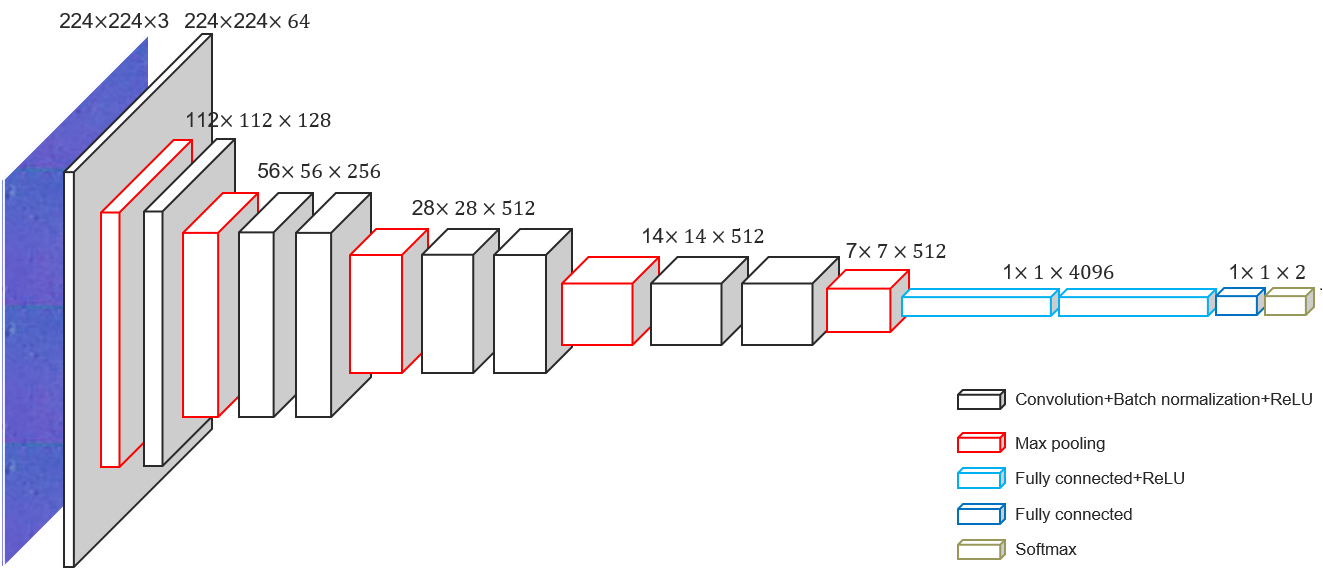
\includegraphics[width=1.0\linewidth]{figures/VGG.png}
\caption{VG-11模型结构示意图}
\label{fig:VGG}
\end{figure}

在训练阶段,我们使用$dropout$方法来预防过拟合。
$Dropout$在向前传播时对神经元以一定的概率随机失活,这种失活只是暂时的,
每一轮训练时,都会以固定的概率重新失活神经元。
本文中$Dropout$失活概率取0.5。


\section{数据预处理}

同基于传统方法的缺陷检测一样,在使用深度学习进行缺陷检测时,数据的预处理也是非常重要的一环。
本章中的数据预处理方法和第\ref{chapter:chuantongfangfa}章类似,
我们首先提取零件的主表面,
接着用数据增强的方法扩大数据规模。

在提取零件主表面阶段,我们使用的方法没有任何变化,此处不再赘述。
在数据增强阶段,我们同样首先对数据做分割,
接着使用镜像和旋转增加样本数量,
但是VGG-11的输入是$224\times 224$,
同\ref{subsubssection:chuantongfenge}节中描述的图像分割方法不同,
本节中滑动窗口的大小为$40\times 40$,
接着我们使用双三次插值法将其放大为$224\times 224$。

\section{模型训练}

在训练阶段阶段,
首先,
我们用\ref{subsection:jilianjianceqi}中提到的方法
将数据集划分为不同的子数据集,
对每个子数据集训练一个VGG-11模型,
最后使用级联的方式将其组合成一个级联检测器。
在模型训练时,
首先初始化模型,
然后优化参数,
直到模型收敛。
初始化模型时,
我们选择在ImageNet上预训练好的参数权重初始化模型。
在优化参数时,
优化的目标函数为\ref{subseciont:sunshihanshu}节定义的损失函数,
在每一轮迭代时,使用$mini-batch$对模型训练,$mini-batch$的大小设置为48,
并使用Adam算法对模型进行优化。
需要注意的是,我们并非选择收敛后的模型作为最终模型,
而是边训练边对模型进行评估,选择测试集上效果最好的模型作为最终模型。


\section{实验结果}

本节将展示使用本章算法进行缺陷检测得到的结果,并将其与传统算法进行对比。
实验使用的深度学习框架是P	ytorch,
该框架是深度学习中常用的框架之一,它能够支持多种平台,现已被广泛应用于学术界和工业界中。

同基于传统方法的缺陷检测算法一样,
我们使用
召回率($REC$)、
查准率($PRE$)、
漏检率( $MDR$)、
误检率($FDR$)
作为模型评价标准,
,其结果如表\ref{tab:shenduxuexijieguo}所示。我们发现,本章算法的实验结果并不比使用HOG、Gredient和RGB联合特征训练出来的传统模型的结果好,我们认为最主要的原因有两点:首先在VGG-11中,输入数据的大小为$224\times 224$,虽然这是原始数据放大之后的结果,但由于缺陷目标往往较小,在这样的输入中,缺陷目标所占比例很小,而模型网络又比较深,使得缺陷区域的特征在最后的特征层中占比更小;其次,受限于缺陷零件数据量,模型容易过拟合。
\begin{table}
\centering
\begin{tabular}{cccccp{38mm}}
\toprule
\textbf{输入类型} & \textbf{REC} & \textbf{PRE} & \textbf{MDR} & \textbf{FDR}\\
\midrule
\mbox{HOG+Gredient+RGB} & 0.9915 & 0.8158 & 0.0085 & 0.0400\\
\mbox{VGG-11} & 0.9643 & 0.7297 & 0.0356 & 0.1786\\
\bottomrule
\end{tabular}
\caption{深度学习和传统方法检测结果表}
\label{tab:shenduxuexijieguo}
\end{table}

在检测速度方面,深度学习由于其复杂的网络结构和较多的网络参数,速度并不快,但由于深度学习和传统方法的输入大小不同,此处并不对其进行比较。


%总结与展望

\chapter{总结与展望}

本章首先对本文工作进行总结,介绍本文工作内容以及创新性,接着提出本文研究的不足和可以改进的地方,对未来的研究工作进行展望。

\section{本文工作总结}

在缺陷检测中,传统的方法对特征选择要求严格,算法容易受各种条件影响,深度学习算法对数据量要求较大,时间复杂度高,并且对小物体检测效果不理想,
而零件的缺陷检测则具有缺陷数量较少、体积较小的特点,直接使用传统算法和深度学习算法都不能得到较好结果。

本文针对这一问题,提供了一种获取零件表面法线信息的算法,该算法使用不同方向光源下拍摄得到的零件图片作为输入,基于光线的反射原理计算零件表面法线。为了获取不同方向光源下的零件照片,我们设计了一套硬件设备,该设备包括遮光模块、平台模块、灯光模块、拍照模块和控制模块五大模块,这些模块将相机、步进电机、LED灯带、滑轨、偏光镜和滤光膜等不同硬件组合成一个整体,从而可以捕获不同方向光源下的零件照片。
同时,在计算表面法线之前,本文首先对相机进行了校正,这些校正包括白平衡校正、色彩校正、畸变校正,
接着对方向光源产生的损失进行了光线补偿,该补偿算法预存储了一套补偿数据,并利用预存储的补偿数据对新的照片进行光线补偿,这些校正和补偿算法极大地改善了设备本身存在的问题,提高了零件法线的精度。
可以从实验结果看到,我们提取出来的法线结果非常精细,较好的还原了物体本身法线。
并且值得一提的是,这一法线提取算法不仅可以用来获取零件法线,也可以用来获取其他物体的法线。

接着本文将法线图作为缺陷检测的输入,验证了其可行性和有效性。在将法线图应用的传统的检测方法时,我们首先对数据做了预处理,根据零件本身特点对图片做展开和截取,从而获得了零件主表面,有效去除了图片背景信息。
接着针对零件缺陷检测中缺陷数据规模小的问题,我们进行了数据增强,使用滑动窗口、旋转、仿射变换等方式扩充了数据规模。
在图像特征提取阶段,我们分别提
取了 Haar-like 特征、图像梯度特征、LBP 特征、GLCM 特征、HOG 特征等
不同的图像特征,用于后续分类,并分析了不同特征的分类效果,根据分
类效果对特征进行组合,从而得到一组最适合这一问题的特征组合。
在分类器分类阶段,我们通过
随机抽样的方法将数据集划分为不同的子集,划分后的每个子数据集中的
样本是均衡的,对于每个数据集,我们选择支持向量机作为基础分类器,
训练多个不同的基础分类器,然后利用 Adaboost 的方法将其组合成一个强
分类器,最终,每个子数据集都可以得到一个强分类器,我们将这些强分
类器利用级联的方式做检测。这种分类器的设计方法不仅能够有效解决数据不平衡的问题,而且可以提高算法的性能和泛化能力。
除此之外,我们还直接使用零件照片训练了传统分类器,分析了它的结果,并将其结果与本文方法的结果进行了对比,这一对比证明了本文方法的有效性。

最后,本文还将法线图作为深度学习模型的输入,训练了一个基于深度学习的目标检测模型。
在使用深度学习模型时,我们同样对数据做了一定的预处理和增强,去除了背景的影响,增加了数据量。
在模型设计阶段,我们针对本文问题对模型进行了修改和优化。
首先,我们调整了模型最后的分类层,改写了损失函数。其次我们向模型中加入了Batch Normalization,
加快了模型收敛速度,
并且可以有效防止过拟合。
最后我们将数据集划分为不同的子数据集,训练了多个模型,
并用级联的方式将这些模型组合成级联检测器,
在解决了数据不平衡问题的同时,提高了模型的效果。
我们将深度学习模型的检测结果与传统检测方法的检测结果进行对比,分析
了二者各自的优缺点及原因。


\section{未来工作展望}

本文虽然取得了一定进展,但是仍有很多可以改进的地方。

首先在零件的法线提取工作中,由于零件本身存在一定厚度,在方向光源照射时会产生阴影。本文并没有考虑阴影对结果的影响,这导致零件法线中部分边缘区域的结果并不理想,因此,这是一个需要继续优化的地方。

其次是在基于传统的缺陷检测算法中,因为数据规模的限制,本文将零件缺陷检测作为一个二分类问题,数据被分为有缺陷和没有缺陷两类。但是在实际的生产环境中,缺陷被分为裂纹、起皮、拉线、划痕、凹坑、凸起、斑点、腐蚀等多类,因此,在获得更多数据之后,我们可以将二分类问题扩展到多分类中去,得到一个更加完善的检测模型。

最后在深度学习算法中,目前已有很多端到端的目标检测算法,比如Yolo、SSD等,但是考虑到这些模型的复杂度和我们目前拥有的数据规模,我们并没尝试这些算法,而是在分类模型的基础上,利用滑动窗口选择候选区域做分类的方法来达到目标检测和定位的效果,我们计划在接下来的工作中使用端到端的方法进行目标检测。


%致谢
%%%%%%%%%%%%%%%%%%%%%%%%%%%%%%%%%%%%%%%%%%%%%%%%%%%%%%%%%%%%%%%%%%%%%%%%%%%%%%%
% 致谢,应放在《结论》之后
\begin{acknowledgement}

从选择了读研,到如今论文完成,时光转眼走过三年。这三年来,有数不清的欢笑与汗水,感动与收获,有太多的人需要我去感谢!

首先,最需要感谢的是我的导师郭延文教授。在论文的编写中,郭老师不仅在选题上给予了我悉心的指导,更是在实验和撰写过程中给出了独特的意见和帮助。作为一名教授,郭博士在学术上拥有极高造诣,是我学术道路上的引路人和指导者,作为一名老师,郭老师以身作则,以严谨的态度和勤奋的精神树立了了我工作、学习和生活上的典范。从老师那里,我得到不仅仅是宝贵的知识财富,更是受益一生的做人道理。

我还要感谢周文喆师兄和吕高建师姐,我们 一起设计了获取物体表面材质的设备,并实现了相关算法,这一过程工程量庞大,仅凭我一人之力可能难以完成,是和他们的通力合作,才完成了这一工作任务,在和他们的合作中我也学到了很多的知识,获得了快速的成长。我要感谢张扬师兄,在将法线信息应用到目标检测的过程中,他以渊博的学术见解和深厚的编程功底为我提供了极大的帮助。感谢同门的于霄和黄凯同学,我们同一级入学,一起学习和生活了诸多时间,这些时间带给我非常多的帮助、快乐和感动,并且在最后的论文撰写和修改阶段,我们互帮互助,顺利完成了各自的论文。感谢你们。

感谢刘明明、朱捷、潘飞、强玉庭、张宏杰、贺敬武五位博士师兄在三年来的帮助和指导,感谢马晗师兄的热心帮助,感谢张可心师妹、张云峰师弟、陈钊民师弟、韩旭师妹,感谢张慧明师弟、陈玉念师妹、罗曼琳师妹、徐春雷师妹,感谢能够相遇在实验室的所有人,感谢你们。

感谢我的舍友孙佳俊、宋仁杰,三年的舍友情弥足珍贵,感谢在南京大学遇到的熊宇、王铖燕等所有的朋友们,是和你们的相遇填满了我研究生生涯的宝贵时光,感谢你们。

最后,我要感谢我的家人,感谢家人给予我的关心与照顾,是他们的支持和陪伴,让我有勇气和力量一路走下去,感谢你们,我爱你们。

感谢!




\end{acknowledgement}


%%%%%%%%%%%%%%%%%%%%%%%%%%%%%%%%%%%%%%%%%%%%%%%%%%%%%%%%%%%%%%%%%%%%%%%%%%%%%%%
% 附录 被我删了不用写


% 参考文献。应放在\backmatter之前。
% 推荐使用BibTeX,若不使用BibTeX时注释掉下面一句。
\nocite{*}
\bibliography{grepaper.bib}

%%%%%%%%%%%%%%%%%%%%%%%%%%%%%%%%%%%%%%%%%%%%%%%%%%%%%%%%%%%%%%%%%%%%%%%%%%%%%%%
% 作者简历与科研成果页,应放在backmatter之后
\begin{resume}
% 论文作者身份简介,一句话即可。
\begin{authorinfo}
\noindent 宋佳,男,汉族,1993年4月出生,山东省枣庄人。
\end{authorinfo}
% 论文作者教育经历列表,按日期从近到远排列,不包括将要申请的学位。
\begin{education}
\item[2015年9月 --- 2018年6月] 南京大学 计算机科学与技术系 \hfill 硕士
\item[2011年9月 --- 2015年6月] 山东大学 软件工程学院 \hfill 本科
\end{education}
% 论文作者在攻读学位期间所发表的文章的列表,按发表日期从近到远排列。
\begin{publications}
\item 宋佳,张扬,郭延文。
发明专利:一种基于深度学习和法向图的零件缺陷检测和定位方法。
中国发明专利(专利申请号:201810063526.2)
\item 宋佳,黄凯,郭延文,曹俊,张琦。
发明专利:一种虚拟现实移动端中基于
矩阵逆运算的图像扭曲方法。
中国发明专利(专利申请号:201610475529.8) 
\item 吕高建,宋佳,郭延文。
发明专利:一种提取材质表面几何和光照物理属性的方法。
中国发明专利(专利申请号:201611183836.5)
\end{publications}
% 论文作者在攻读学位期间参与的科研课题的列表,按照日期从近到远排列。
%\begin{projects}
%\item 国家自然科学基金面上项目``无线传感器网络在知识获取过程中的若干安全问题研究''
%(课题年限~2010年1月 --- 2012年12月),负责位置相关安全问题的研究。
%\end{projects}
\end{resume}

%%%%%%%%%%%%%%%%%%%%%%%%%%%%%%%%%%%%%%%%%%%%%%%%%%%%%%%%%%%%%%%%%%%%%%%%%%%%%%%
% 生成《学位论文出版授权书》页面,应放在最后一页
\makelicense

%%%%%%%%%%%%%%%%%%%%%%%%%%%%%%%%%%%%%%%%%%%%%%%%%%%%%%%%%%%%%%%%%%%%%%%%%%%%%%%
\end{document}
